\documentclass{article}
 \usepackage[table,xcdraw]{xcolor}
%\documentclass[twocolumn,showpacs,showkeys,preprintnumbers,amsmath,amssymb]{revtex4}
\usepackage[american]{babel}
\usepackage[latin1]{inputenc}
\usepackage{graphicx}
\usepackage[colorinlistoftodos]{todonotes}
\usepackage{booktabs}
 \usepackage{booktabs}
\usepackage{float}
\usepackage{subcaption}
\usepackage{indentfirst}
\usepackage{natbib} 
\begin{document}


\title{Some title}

%\vspace{1cm}

\author{Marcelo V. Maciel \and Andr\'e C. R. Martins\\
	%}
	%\email{amartins@usp.br}
	%\affiliation{%
	NISC - EACH, Universidade de S\~ao Paulo\\
	Av. Arlindo B\'etio, 1000, S\~ao Paulo, 03828-080, Brazil}

%\author{Andr\'e C. R. Martins\\
	%}
 %\email{amartins@usp.br}
 %\affiliation{%
%NISC - EACH, Universidade de S\~ao Paulo\\
%Av. Arlindo B\'etio, 1000, S\~ao Paulo, 03828-080, Brazil}
 

\date{}


\maketitle
%\vspace{0.3cm}

%\center{\Large\bf Segundo autor}
%\center{\large\bf Afilia��o}


\begin{abstract}
	
	
	%\keywords{}
	%\pacs{}
\end{abstract}


\section{Introduction}

 % Incluir aqui a parte sobre teoria pol�tica, um par�grafo � suficiente, a princ�pio.

Here, we will present an opinion dynamics model
\cite{castellanoetal07,galam12a,galametal82,galammoscovici91,sznajd00,deffuantetal00,martins08a}
where the opinions exist over an one-dimensional axis and each agent has a best
estimate on more than one issue over that axis. Describing opinions over a
spatial landscape is an usual way to describe policy alternatives and agents'
preferences. The geometrical properties of the space are usually defined by
mapping from similarity to proximity of the political agents
\cite{downs1957economic, laver2014measuring}. Such a description can capture the
common notion of parties or policies being more ``to the left'' or ``right''. If
they're similar then they're closer \cite{van2005political, miller2015spatial}.
Major opinions, including political ones, tend to be formed not from only one
issue but from how each person feels about a number of them. Locating someone in
a left versus right or liberal versus conservative axis, therefore, requires
inspecting the opinions of that person in not only one but several issues that constitute the agent ideological positioning \cite{benoit2006party}.

For many problems, it makes sense to consider different issues as having components in
more than one single dimension \cite{vicenteetal08b}. However, it is often the case that describing the problem as
one-dimensional can be justified. We can certainly see this as a
first approximation along the most relevant dimension. In that case, the one dimensional case is
just a projection along a direction where variation seems especially important of higher-dimensional problems. From an application point of view, it is usual to find discussions to be simplified over only one main disagreement.  

One traditional way to model this type of scenario is to use continuous opinions
over a fixed interval, as it is done in the Bounded Confidence (BC) models
\cite{deffuantetal00,hegselmannkrause02}. While discrete models
\cite{galametal82,galammoscovici91,sznajd00} can be very useful at describing
choices, they are not easiest way to represent strength of opinion unless a
continuous variable is associated to the choice \cite{martins08a}. Discrete
models also tend to lack a scale where we can compare opinions and decide which
one is more conservative or more liberal.

On the other hand, continuous models are not particularly well suited for
problems involving discrete decisions. As we will not deal with those kinds of
problems here, they are a natural choice. Indeed, continuous opinions models
have been proposed for several different problems on how opinions spread on a
society \cite{deffuantetal02a,weisbuchetal05}, from questions about the spread
of extremism
\cite{amblarddeffuant04,gargiulomazzoni08a,franksetal08a,alizadeh14a,Albi2016,Mai2017}
to other issues such as how different networks
\cite{Kurmyshev2011,Acemoglu2011,Das2014,Hu2017} or the uncertainty of each
agent \cite{deffuant06} might change how agents influence each other.

Here, we will use a continuous opinion model created by Bayesian-like reasoning
\cite{martins08c}, inspired by the Continuous Opinions and Discrete Actions
(CODA) model \cite{martins08a,martins12b}. That model was shown previously
\cite{martins08c} to provide the same qualitative results as BC models. While a
little less simple, the Bayesian basis makes for a clearer interpretation of the
meaning of the variables. That makes extending the model and interpreting new
results simple. That approach is also consistent with a bounded rationality
variant interpretation of the spatial model of political decision making
\cite{humphreys2010spatial,ostrom1998behavioral}.

Variations of how each agent estimate how trustworthy other agents are will also
be introduced. Here, we use a function of trust $p^*$ that plays a role similar
to the threshold value in BC models. While $p^*$ is not a simple discontinuous
cut-off, it is a function of the distance between the opinions of the agent and
the neighbor. If only one issue is debated, that distance is uniquely defined.
However, if we have multiple issues represented on the same one-dimensional
line, it is not clear which distance we should use. That happens because we have
the opinion of agent $i$ on a specific issue $o_i$ and we can compare it to
$o_j$ to estimate how much $i$ trusts $j$. However, as there are several issues
we could also use the mean opinion of $i$ over all its issues and the same goes
for $j$. Therefore, we will study two additional cases: in the first
alternative, we will change \(p^*\) to \(p^{**}\), determined by the distance
between the neighbor and the agent average opinions. In the second alternative,
we will use a \(p^{***}\) calculated from the opinion of the neighbor and the
average opinion of the agent. The idea here is to make the behavior of our
agents closer to what experiments show about human reasoning. We have observed
that our reasoning about political problems can be better described as
ideologically motivated \cite{jostetal03a,taberlodge06a,Claassen2015a}. Indeed,
our opinions tend to come in blocks even when the issues are logically
independent \cite{jervis76a}. Our reasoning abilities seem to exist more to
defend our main point of views \cite{mercier11a,merciersperber11a} and our
cultural identity \cite{kahanetal11} than to find the best answer. In that
context, evaluating others by how they differ from us as a whole, instead of in
each issue, is a model variation worth exploring.
 
\section{The Model}


Here, the population will consist of  \(N\) agents fully connected (an agent $i$ can interact with any other agent $j$). Each agent $i$ will have an opinion $0\leq o_{i,k} \geq 1$, where $k=1, \ldots, n$ is a specific issue. We assume each agent opinion about issue $k$ can represented as a value $o_{i,k}$ at the range of possible values for $o$s. Agents also have an uncertainty $\sigma$ associated to their average estimate $o$. The uncertainty $\sigma$ could be different for each agent and also updated during the interactions \cite{martins08c}. For the sake of simplicity, however, we will assume the uncertainty $\sigma_i =\sigma$ is identical for (almost) all agents and it does not change. The set of opinions for each agent on all possible issues will define its ideological profile
\(I_i
=
(
(o_{i, 1}, \sigma),
\ldots,
(o_{i, n}, \sigma)
)
\)
, where \(n\) is the number of issues, \(o\) is
the opinion about the issue and \(\sigma\) is the global  uncertainty~\cite{martins12b}. The arithmetic mean  $x_i$  of agent $i$ opinions in each issue will be called here the ideal point for each agent, that is, it defines the agent ideological position at the
dimension of interest \cite{armstrong2014analyzing}. Obviously
\(
x_i
=
\frac{1}{n}
\sum_{k=1}^{n}
o_{k}
\).


In order to have agents with initial ideal points well distributed over the
possible range, the initial valued for each \(o_{i, k}\) was randomly drawn
using a Beta \(Be(\alpha, \beta)\) with random parameters $\alpha_i$ and
$\beta_i$. Those parameters were drawn for each agent $i$ from the ranges \( (
\alpha \in [1.1, 100], \beta \in [1.1, 100] ) \) by dividing those ranges by
\(N\) equally spaced values and then assigning them to each agent after mixing
the values as in a Latin hypercube sampling~\cite{mckay2000comparison}. That is done to
allow agents with a diverse value of initial ideal points and, at the same time,
to keep the initial \(o_{i, k}\)s of each agent $i$ correlated.

While we could have \(\sigma\) as a measurement of each agent uncertainty and have it evolve with time, here we will keep it as a fixed parameter of the model. However, a
proportion \textit{p$\_$intran} of agents will be stubborn about one single issue $k$, so that \(\sigma_{i,k}
= 1e-20\). That behavior is kept constant as the simulation unfolds, that is $\sigma_{i,k}$ is also not updated by the model. A proportion of agents who are stubborn is introduced here so we can check if inflexible \cite{galam05b,deffuant2002can,martinsgalam13a} have a significant impact on the outcomes of the model.


%For its part, \(\sigma\) is a parameter of the model, not the agents. However, a
%proportion \textit{p$\_$intran} of the agents will have an unique \(\sigma_{i,k}
%= 1e-20\). This is done so that we can control for the impact of inflexible
%agents on the model dynamics \cite{galam05b,deffuant2002can,martinsgalam13a}.

%How many agents are intransigent is also a parameter (coded as
%\textit{p$\_$intran} ), and such \(\sigma\) is established at the initial
%condition by sampling the issue index from the \(I_i\)'s length. This means that
%we've opted for an implementation in which agents are intransigents in a
%\textit{single} issue.

In each iteration of the simulation, two procedures are applied: the
opinion update through social influence, and a random opinion update (noise). In
the social influence procedure we draw two agents, \(i\) and \(j\), from the
population, where \(i\) will observe \(j\) opinion about a randomly drawn issue \(k
\in (1 , \ldots, n)\). %That way, we have the corresponding pairs (\(o_{i,k},
%o_{j,k}\)) and (\(\sigma_{i,k}, \sigma_{j,k}\)). 
Agent \(i\)
updates its opinion (\(o_{i,k}\)) following an approximate Bayesian rule. That rule is obtained by assuming each agent has a
Normal prior \(f_i(\theta) = \frac{1}{\sqrt{2 \pi} \sigma_i} e^{- \frac{(\theta
- o_i )^2}{2 \sigma_i}} \) compatible with its parameters $o_{i}$ and $\sigma_{i}$, where the index related to the issue $k$ was omitted for the sake of simplifying the equation.  The agents also assume a mixture likelihood where there is an initial chance
\(p\), updated to \(p^*\) that the agent \(j\) has information and a chance
\(1-p\) it knows nothing and its opinion is just a random non-informative draw. That is, the likelhood is given by
 \( f(o_j|\theta) = p N(\theta,\sigma_j^2) + (1-p)U(0,1) \). While a full Bayesian treatment would produce a posterior distribution that is a mixture of two normals, here we will assume each agent only updates its expected value and it does not carry the full posterior information to the next iteration. That leads to the following update rule for the expected value $o_{i,k}$ \cite{martins12b}:


  \begin{equation}\label{eq:oupdate}
    o_{i,k}(t+1) =
    p^{*}
    \frac{o_{i,k}(t) + o_{j,k}(t) }{2}
    +
    (1 - p^{*})
    o_{i,k}(t),
  \end{equation}
where  $p^{*}$ is given by
  \begin{equation}\label{eq:pstar}
   p^{*}
    =
  \frac{
      p \frac{1}{\sqrt{2 \pi} \sigma_i}
      e^{- \frac{ (\Delta_{ij})^2}{2 \sigma_i^2}}
    }{
      p
      \frac{1}{\sqrt{2 \pi} \sigma_i}
    e^{- \frac{ ( \Delta_{ij})^2}{2 \sigma_i^2}}
    +
    (1 - p)
  }.
  \end{equation}
Here \(\Delta_{ij} = o_{i,k} (t) - o_{j,k} (t)\) is the distance between the opinions on the $k$ issue. $\Delta_{ij}$ plays a
similar role to the threshold parameter in the Bounded Confidence models by making distant opinions less influential. As $\Delta_{ij}$ increases, it is easy to see that Equation\ref{eq:pstar} causes  $p^{*}$ to tend to zero. And, as that happens, the weights in average update Equation~\ref{eq:oupdate} change so that the previous value $ o_{i,k}(t)$ remains almost unchanged.

The threshold role of $\Delta_{ij}$ suggests we might change its definition to check how it might better reflect the actual behavior of humans. In particular, people tend to trust better those who have a similar ideology. That means trust might not depend on the specific issue alone, but on the average over all issues. While that is not the model we obtain from applying Bayes rule, such a change makes sense
as an attempt to have a better model. In order to check that possibility we will also implement two other cases by changing the way $\Delta_{ij}$ is calculated. In the first variation, $p^*$ will be substituted by \(p^{**}\), where \(p^{**}\) means 
 \(\Delta_{ij} = x_i(t) - x_j(t) \), that is, agent $i$ will observe the average
 ideological position of $j$ in order to estimate its trust. That assumed $i$
 has more information than only the value $o_{j,k}(t)$. To check what happens
 when indeed only $o_{j,k}(t)$ \textcolor{red}{indeed what??}\todo[color =
 yellow!20]{take a look at this sentence}, we will introduce a second variant case where $i$ compares $o_{j,k}(t)$ to its own average. That is,  \(\Delta_{ij} = x_{i}(t) - o_{j,k}(t)\) and we represent that case by \(p^{***}\).

In order to better understand the model dynamics we also introduce noise as the second procedure. At each iteration, 
another agent \(i\) is randomly chosen and its opinion changed due to random noise. That is, $i$ opinion becomes \(
o_{i,k}(t+1) = o_{i,k}(t) + r \) where \(r\) is drawn from a Normal
distribution with mean 0 and standard deviation \(\rho\). If agent \(i\) is intransigent in
issue \(k\) it won't its \(o_{i,k}\) opinion when chosen by
the noise algorithm. Moreover, if \(o_{i,k}(t) + r > 1\) then \( o_{i,k}(t+1) =
1\). Likewise, if \(o_{i,k}(t) + r < 0 \) then \( o_{i,k}(t+1) = 0\). Noise
is introduced here as a way of accounting for the effect of factors not related to the modeled
social influence \cite{flache2017} and it is interesting to verify if small noises can lead to drastic changes in
systemic properties \cite{macy2015signal}.

  \section{Model Results}

  To better understand the model behavior, we run simulations using as range for the parameters the values:  

  \begin{table}[H]
    \centering
\begin{tabular}{@{}|l|l|l|l|l|l|@{}}
\toprule
\rowcolor[HTML]{EFEFEF} 
$\sigma$ & $n$ & $p$ & $p\_intran$ & $N$ & $\rho$ \\ \midrule
$[0.01, 0.5]$ & $[1, 10]$  & $[0.1, 0.99]$ & $[0.0, 0.1]$ & $[500, 5000]$ & $(0.0, 0.1]$ \\ \bottomrule
\end{tabular}
\caption{Parameters' Bounds}
\end{table}


The parameter space was explored by two sweeps of its parameters: one sampling
of 70,000 times using quasi-random low-discrepancy sequences
\cite{saltelli2008global}, that generate evenly spaced points, and another of
60,000 times keeping \(N=500\) so that we can compare different runs. An
important question in any opinion dynamics model is if agents can reach
consensus. That can be observed by comparing the initial mean (\( \frac{1}{n}
\sum_{k=1}^{n} o_{k} \)) and standard deviation (\( \sqrt{ \frac{1}{n}
  \sum_{k=1}^{n} (o_{k} - x_i)^2 } \)) of each agent's opinions. Figure
\ref{fig:std} shows histograms for these variables at the initial condition and
also for the sets of simulation's end states corresponding to the (\(p^{*},
p^{**}, p^{***}\)) cases.


\begin{figure}[H]
  \centering
  \captionsetup{justification=centering,margin=2cm}
    
    
  \begin{subfigure}[h]{0.85\textwidth}
    
       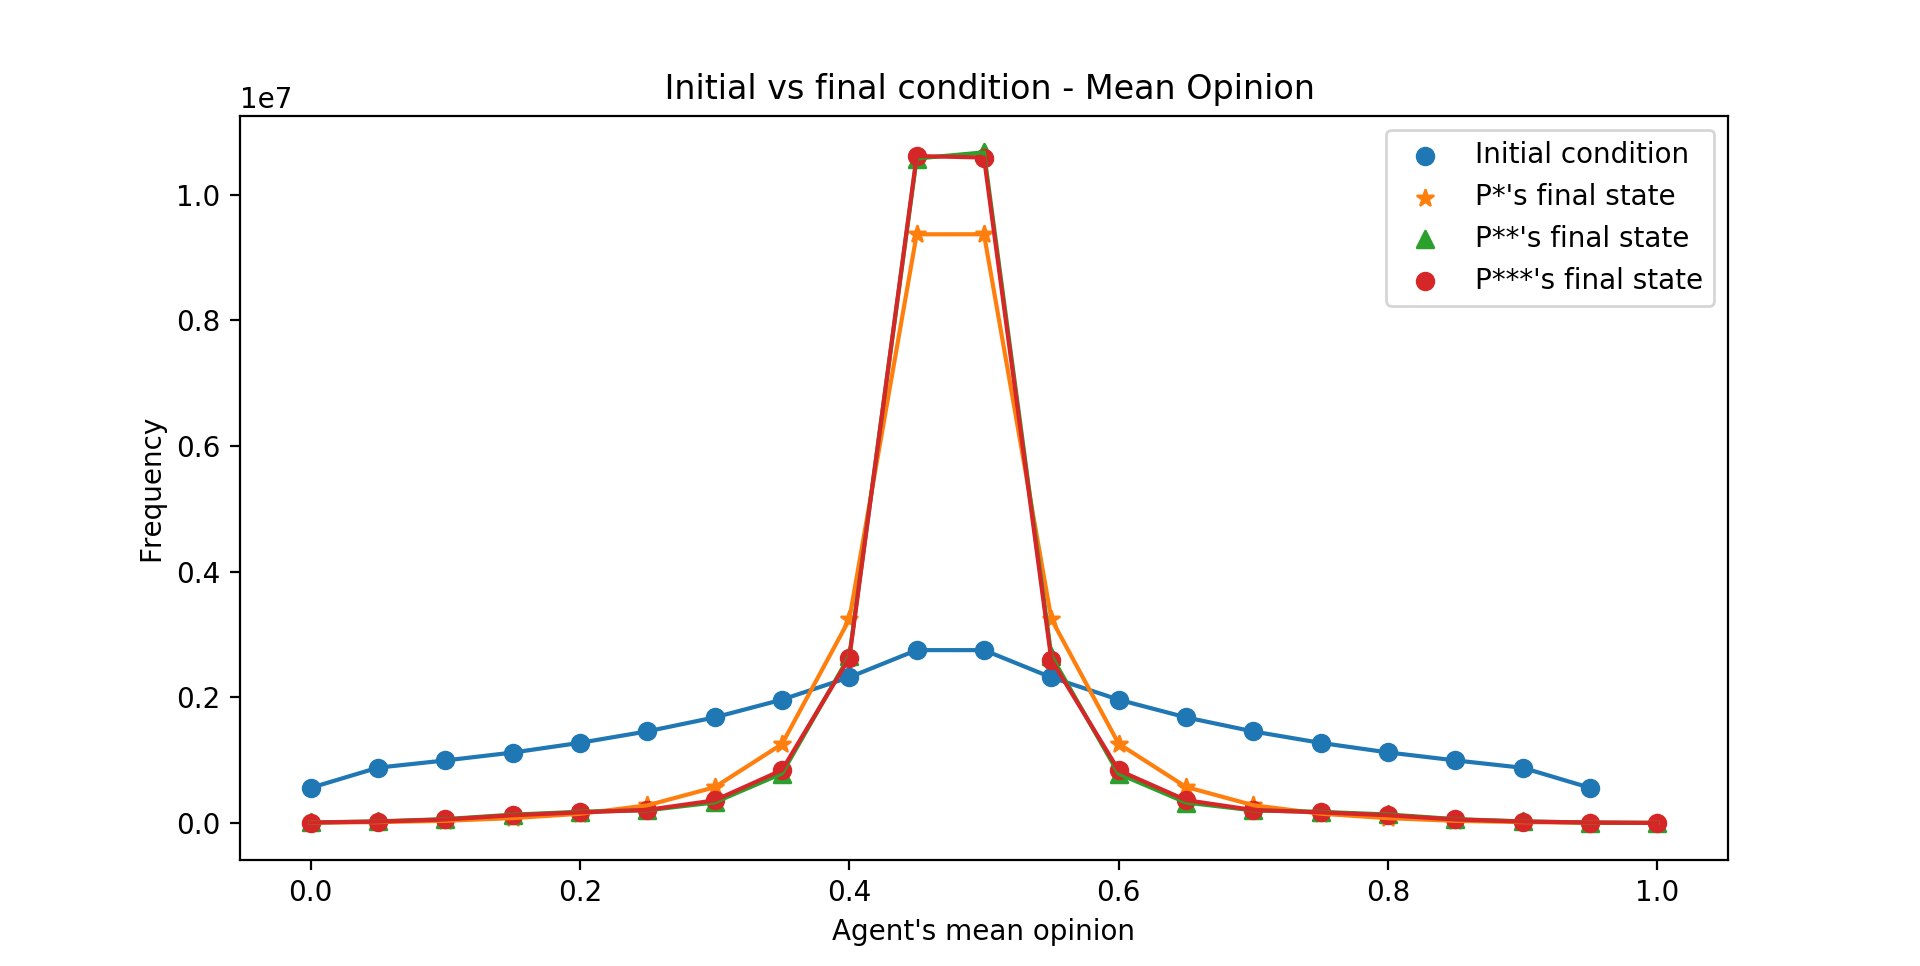
\includegraphics[width=\textwidth]{img/mean_hist.png}
       \caption{Initial x Final state: \\ agents' mean opinions.}
     \end{subfigure}
     \begin{subfigure}[b]{0.85\textwidth}
       
       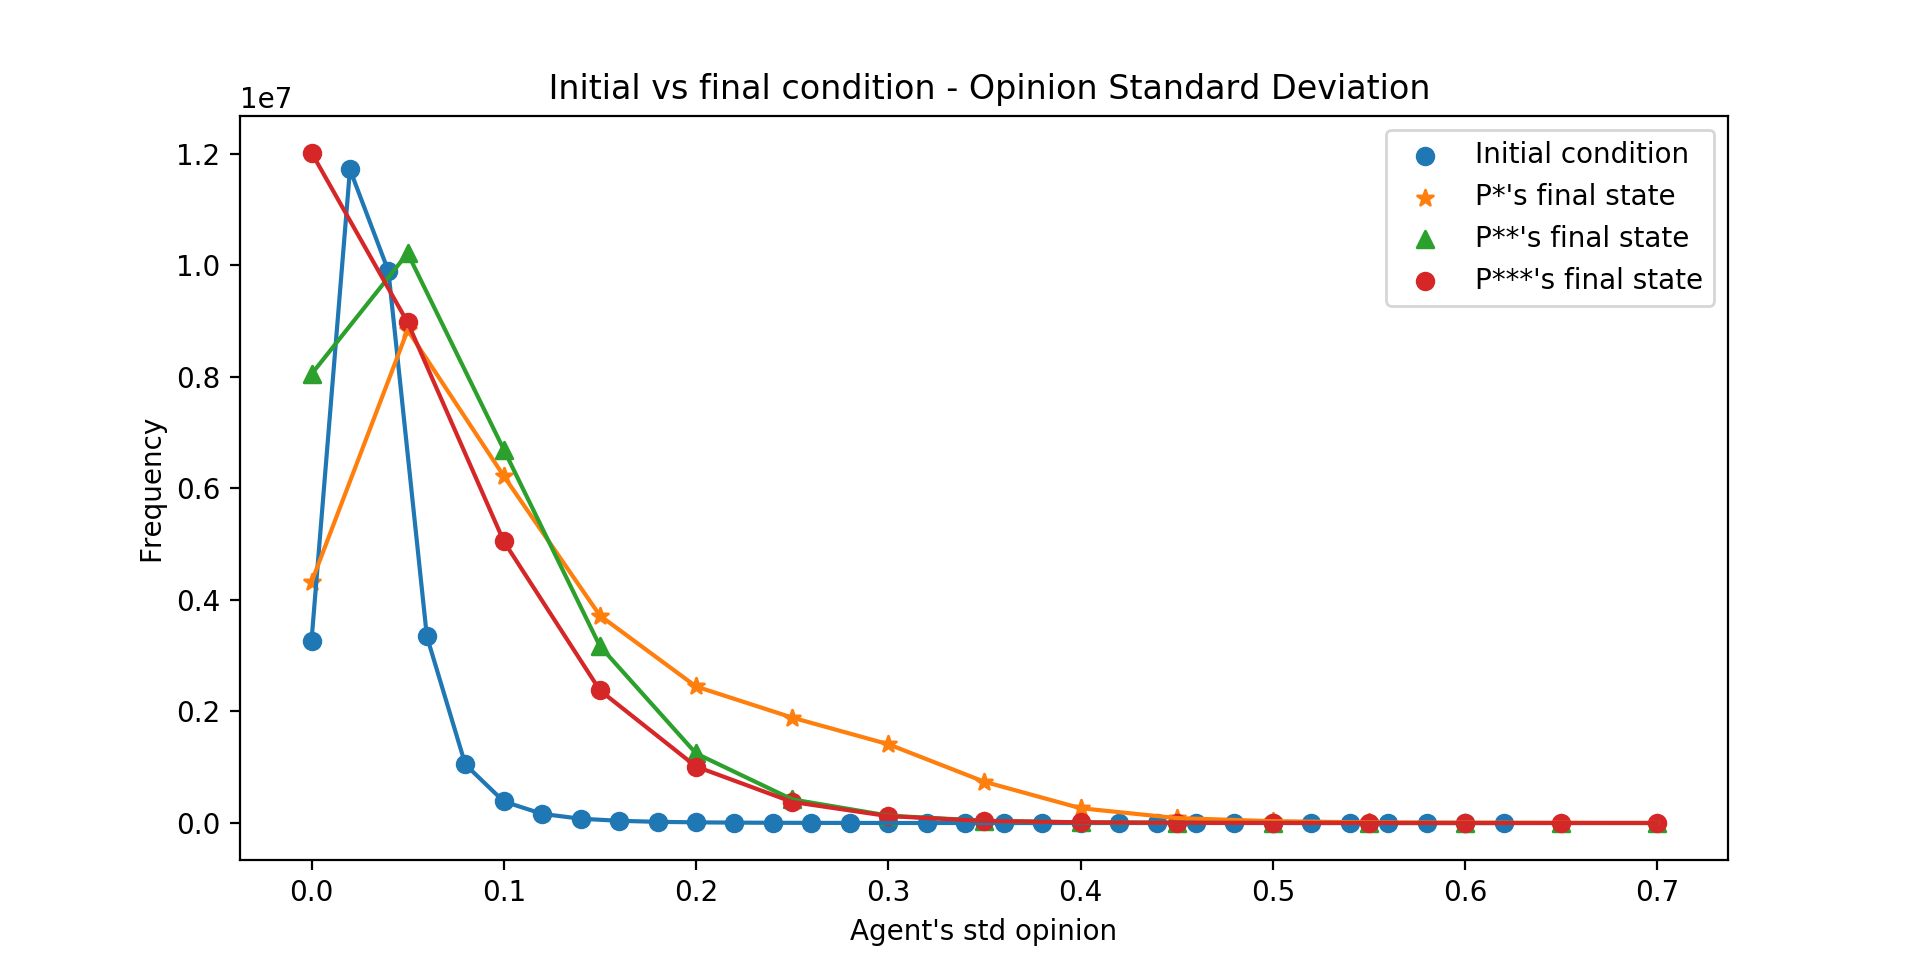
\includegraphics[width=\textwidth]{img/std_hist.png}
       \caption{Initial x Final state: \\ standard deviations of opinions}
     \end{subfigure}
     \caption{Difference for initial and final conditions for 60.000 parameterizations. \(N = 500\)
     for comparability.} 
     \label{fig:std}
    \end{figure}

    The histograms show that, in general, we have a greater central tendency
    than the initial random situation. The peak at the value 0.5 is now ( Figure
    \ref{fig:std} (b)) \(\approx 10^7\) while at the initial condition ((
    Figure \ref{fig:std} (a)) was  \(\approx 5 * 10^5\) while the histograms
    become more centered. This seems to suggest a tendency to consensus in many
    cases. However, consensus is not always achieved, as shown by the tails of
    Figure \ref{fig:std} (b) and since there is also a change at the standard
    deviation distributions ( Figure \ref{fig:std} (c)). That can be explained
    by cases where bi-partisanship becomes stronger, with agents tending to both
    extreme positions. That suggest that, in general, the model can be described
    as one with similarity biased influence \cite{flache2017}.

    \todo[inline]{Ver se consigo descrever os histogramas melhor, agora n�o ta
      saindo.}
    
    The histograms, however, don't show which values of the parameters cause
    those changes. They also say nothing about which parameters are relevant and
    which ones have little influence on the final outcome. With that in mind we
    perform a Sobol sensitivity analysis \cite{saltelli2000sensitivity}. The
    Sobol indexes decompose the impact of parameters on the variance of the
    output. The higher the value of index the bigger the impact of the parameter
    on the output. First order Sobol indexes include linear and non-linear
    contributions of the parameters, while total Sobol indexes also include all
    the interaction effects between parameters \cite{ten2016sensitivity}. If
    there are only three parameters, the total effect \(S_{T1}\) of the first
    parameter \(X_1\) is given by the equation \(S_{T1} = S_1 + S_{12} + S_{13}
    + S_{123}\) where \(S_i = \frac{V[E(Y|X_i)]}{V(Y)}\); \(S_{12}\) is the
    impact at the variance of the output \(Y\) of the interaction of \(X_{1}\)
    and \(X_{2}\); that is, their combined effect minus their first order
    effects: \(S_{ij}\) = \(\frac{V[E(Y|X_i,X_,)] - V[E(Y|X_i)] -
      V[E(Y|X_j)]}{V(Y)} \) \cite{saltelli2008global}. For our simulations, we
    obtain the estimates:

     
    \begin{figure}[H]
  \centering
    \begin{subfigure}[b]{0.45\textwidth}
      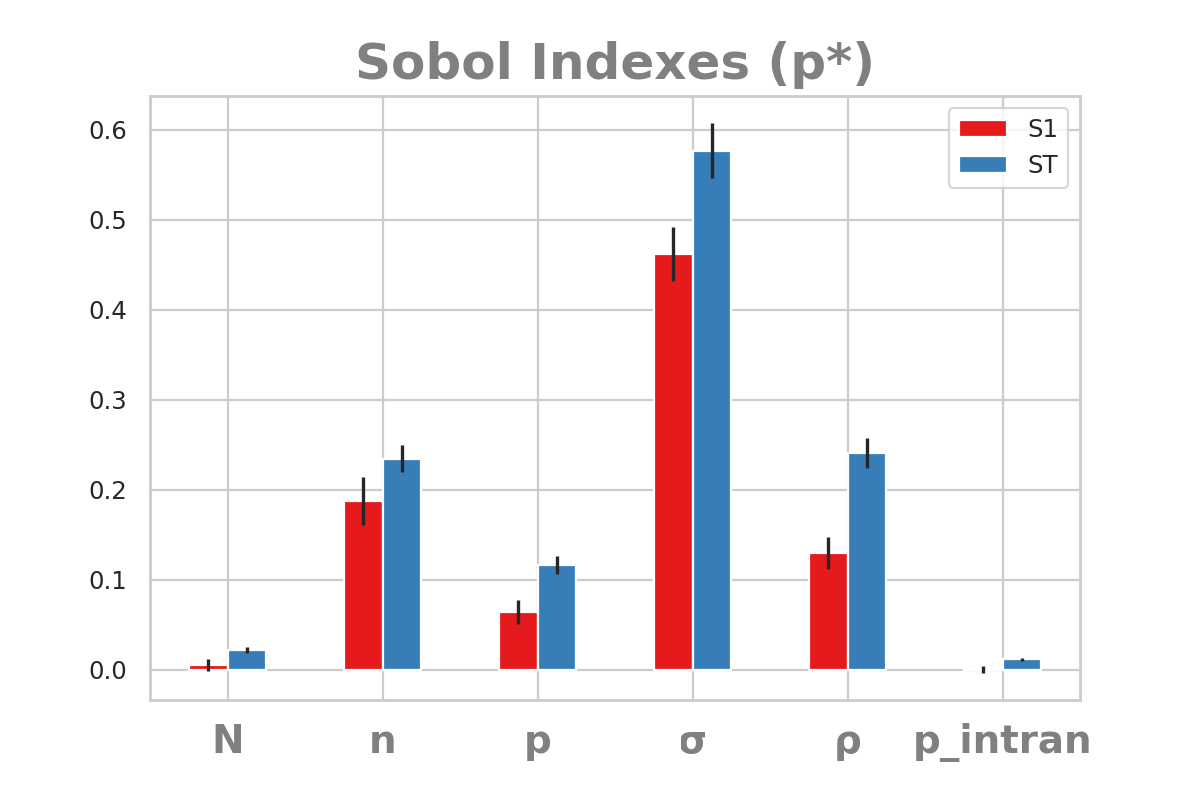
\includegraphics[width=\textwidth]{img/sobolpstar1.png}
%      \caption{\( n\_issues = 1,  \sigma = 0.1\) }
    \end{subfigure}
         \begin{subfigure}[b]{0.45\textwidth}
      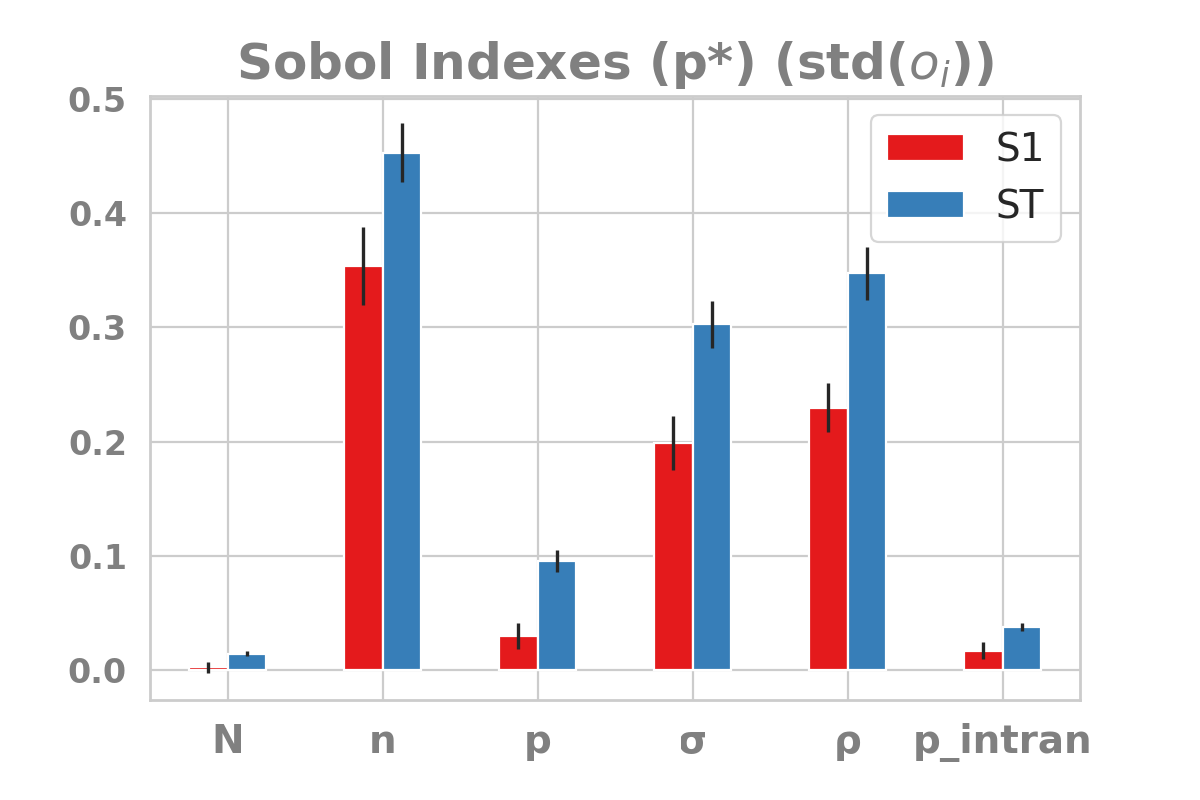
\includegraphics[width=\textwidth]{img/sobolpstar1-measurestd.png}
%      \caption{\( n\_issues = 1,  \sigma = 0.1\) }
    \end{subfigure}
    \begin{subfigure}[b]{0.45\textwidth}
      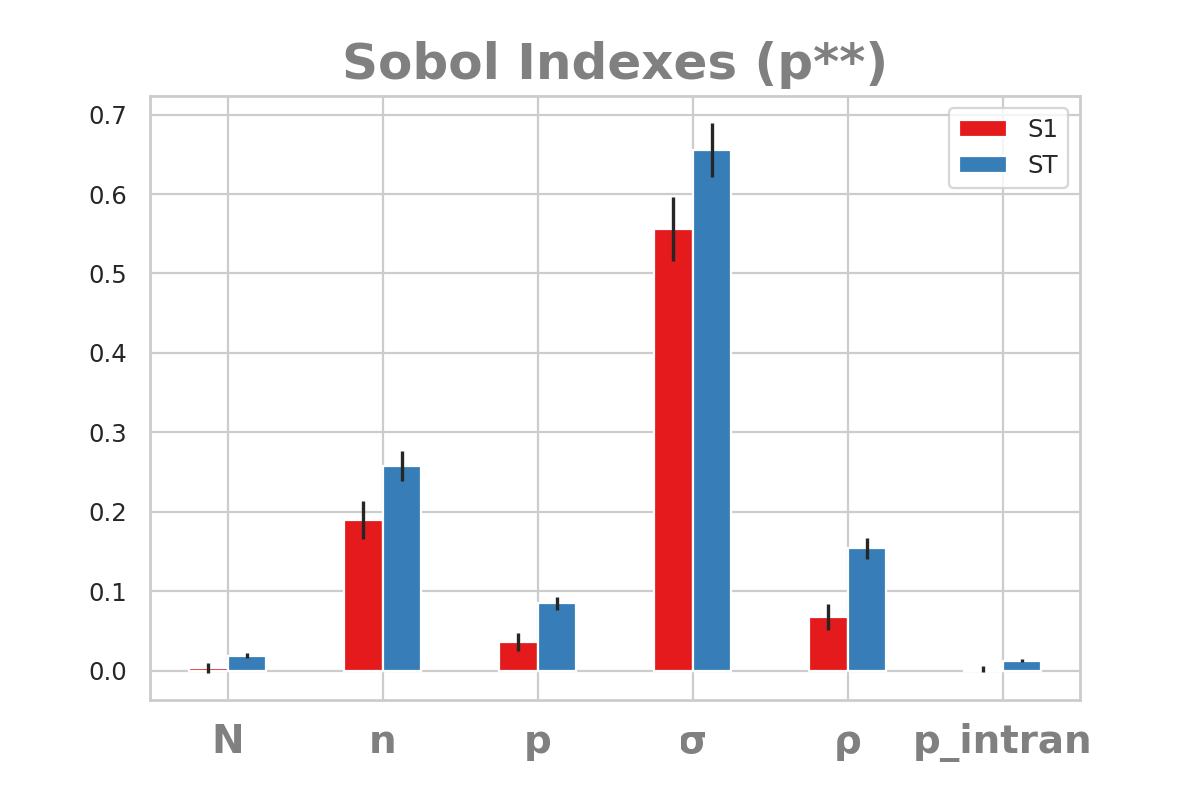
\includegraphics[width=\textwidth]{img/sobolpstar2.png}
 %      \caption{\(n\_issues = 1, \sigma = 0.02\) }
     \end{subfigure}
    \begin{subfigure}[b]{0.45\textwidth}
      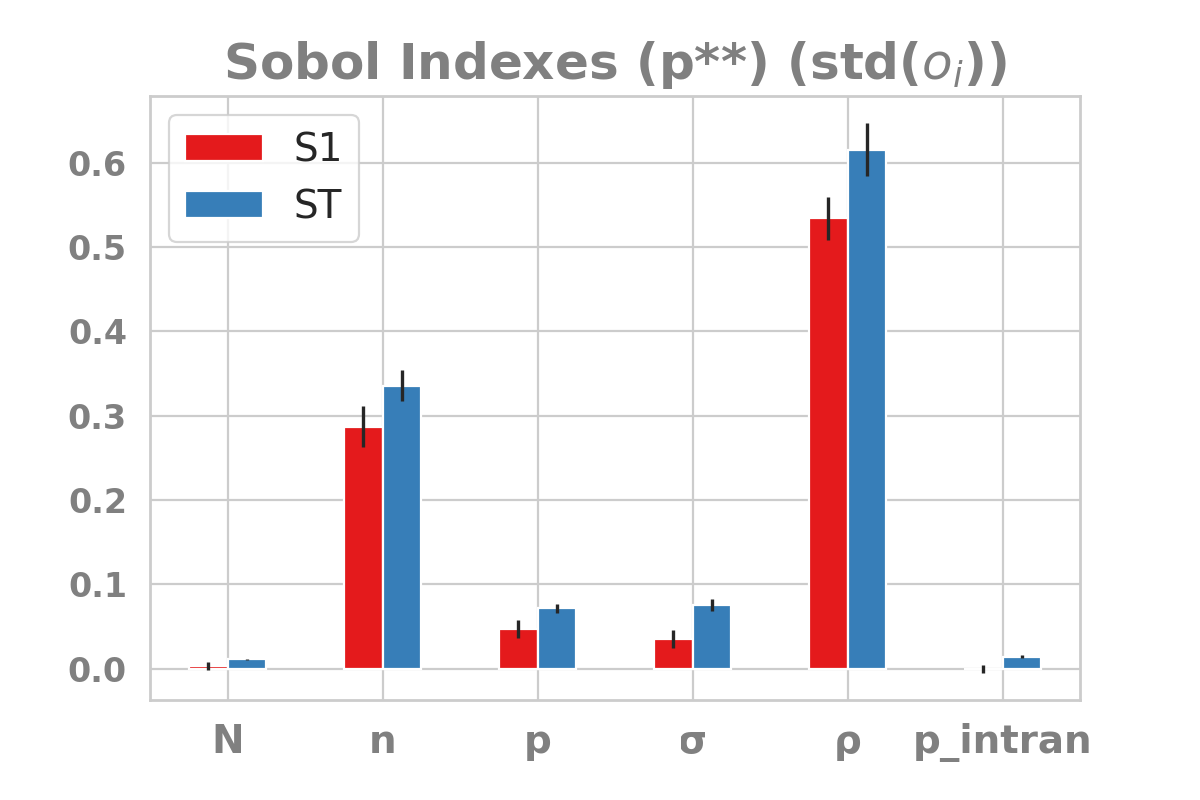
\includegraphics[width=\textwidth]{img/sobolpstar2-measurestd.png}
 %      \caption{\(n\_issues = 1, \sigma = 0.02\) }
     \end{subfigure}
     \begin{subfigure}[b]{0.45\textwidth}
       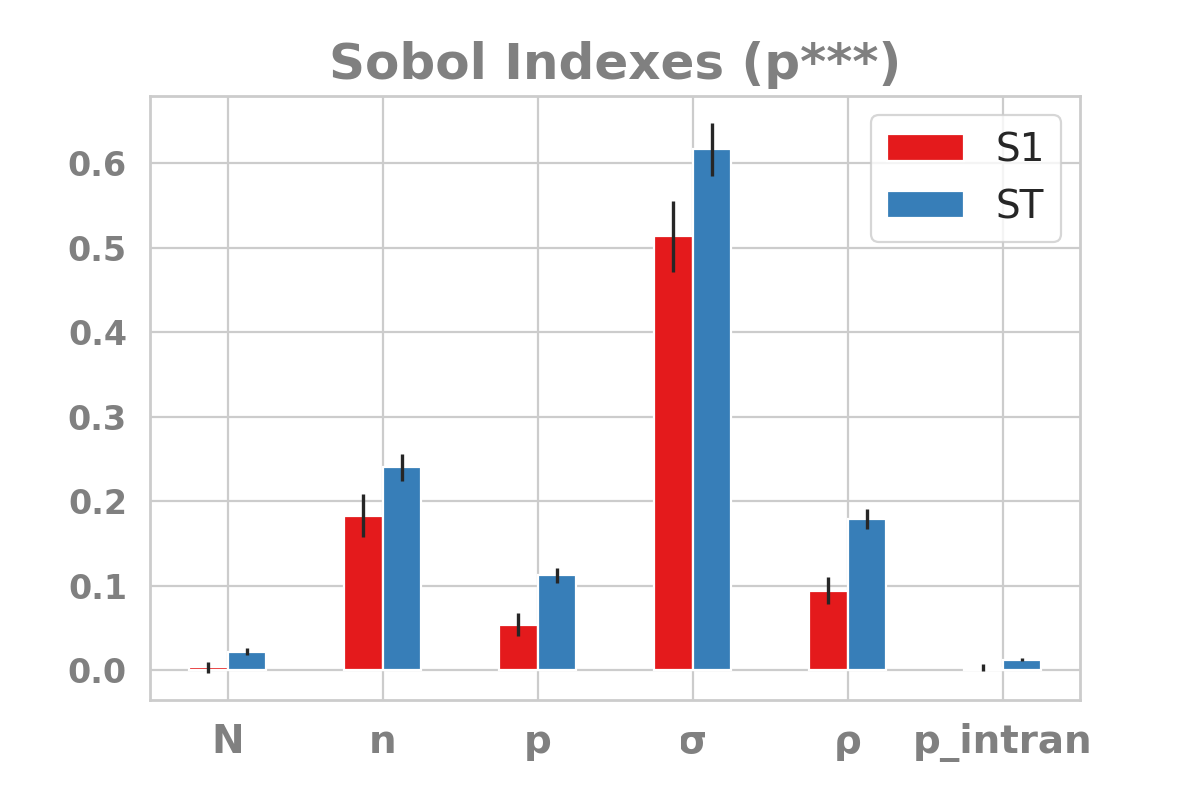
\includegraphics[width=\textwidth]{img/sobolpstar3.png}
  %     \caption{\(n\_issues = 7, \sigma = 0.1\)}
     \end{subfigure}
     \begin{subfigure}[b]{0.45\textwidth}
       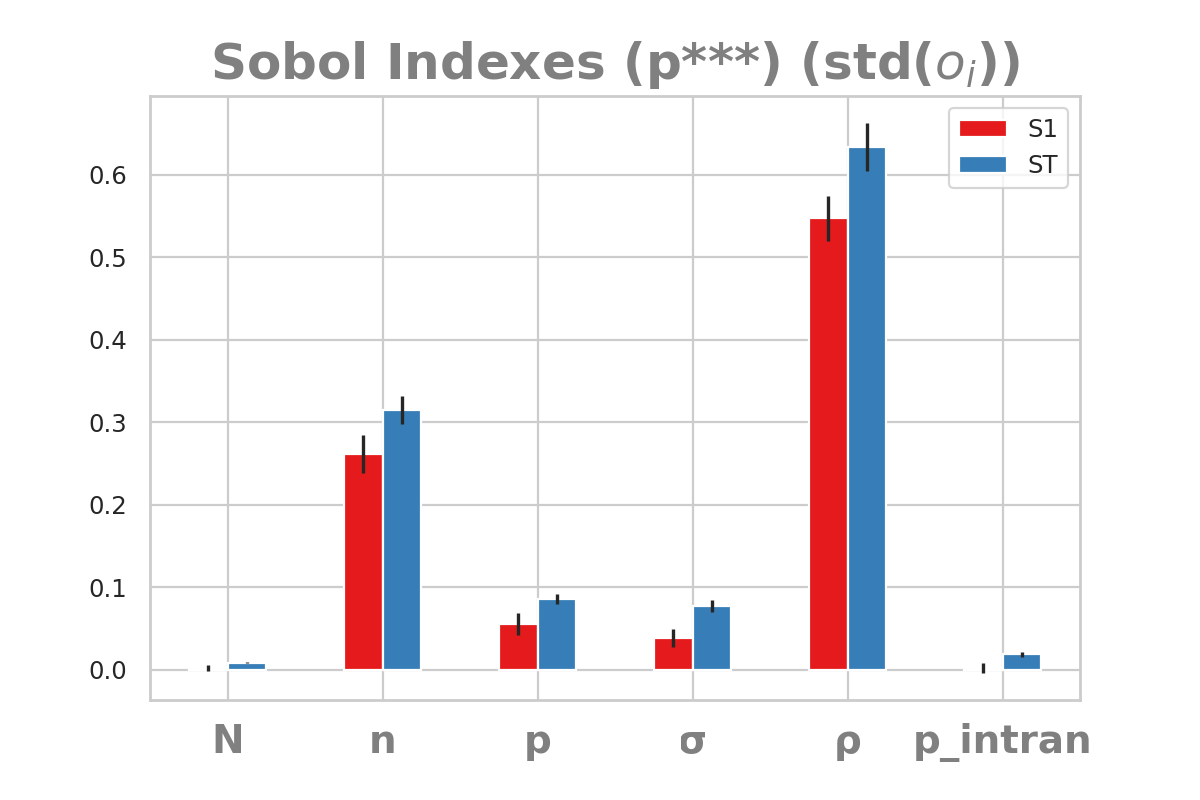
\includegraphics[width=\textwidth]{img/sobolpstar3-measurestd.png}
  %     \caption{\(n\_issues = 7, \sigma = 0.1\)}
     \end{subfigure}
     \caption{Sobol Indexes for the three cases (\(p^{*}, p^{**}, p^{***}\))}
     \label{fig:sobol} 
    \end{figure}

    The sensitivity analysis in Figure\ref{fig:sobol} shows that \(\sigma, n \),
    and \(\rho\) have the most influence on the final values of (\(Ystd\)). $p$
    seems to still have some smaller influence and both $N$ and $p_{intran}$
    seem to make no difference. It is also interesting to notice that the same
    behavior appears in the three. \(\sigma\) being the parameter that explains
    most of the variance was expected and it is consistent with
    \citep{martins12b}. It is interesting to see that two of the new parameters,
    the number of issues $n$ and the noise \(\rho\), also play an important role
    in explaining the total variance.
     
    The
    sensitivity analysis, however, does not show the direction of the impact,
    which we investigate through scatter plots shown in Figure \ref{fig:scatters}. Each value of (\(Ystd\)) in those graphics correspond
    to the outcome of one implementation of the model for the value of the parameter at the $x$-axis.


        \begin{figure}[H]
  \centering
  
    \begin{subfigure}[b]{0.45\textwidth}
      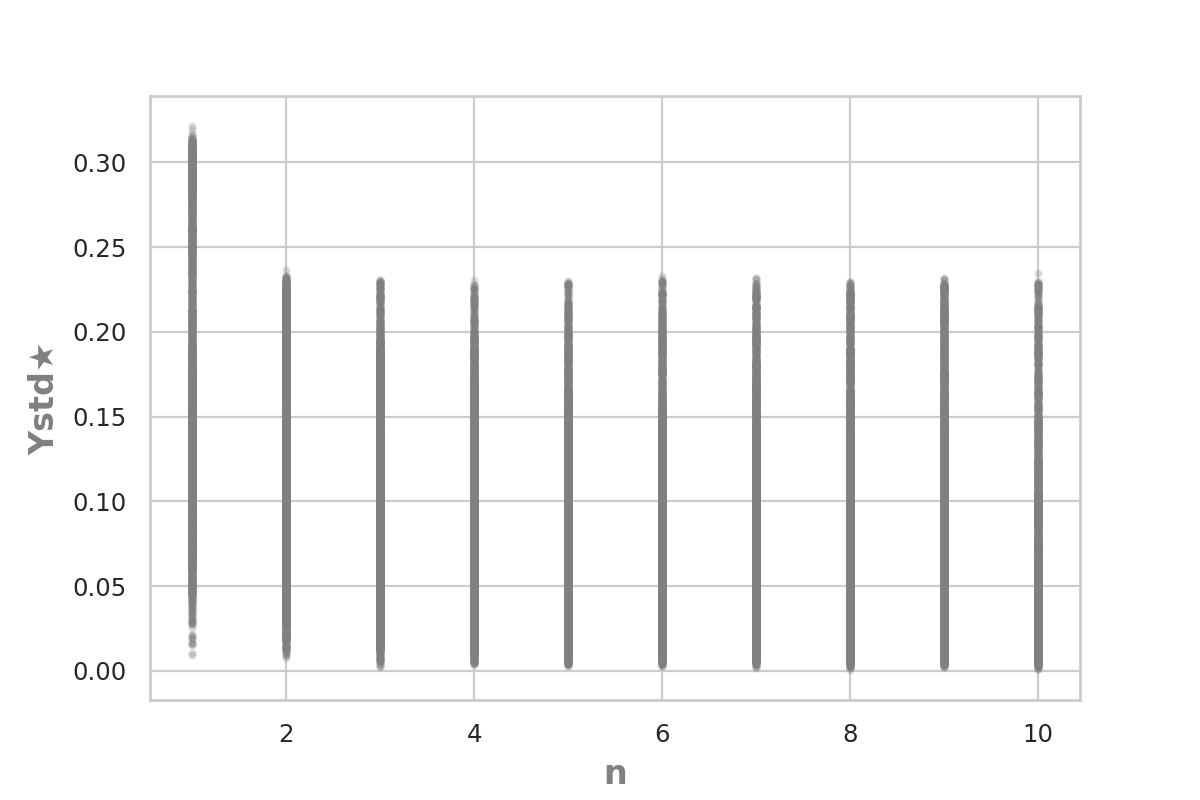
\includegraphics[width=\textwidth]{img/regressionYstd*n.png}
    \end{subfigure}
    \begin{subfigure}[b]{0.45\textwidth}
      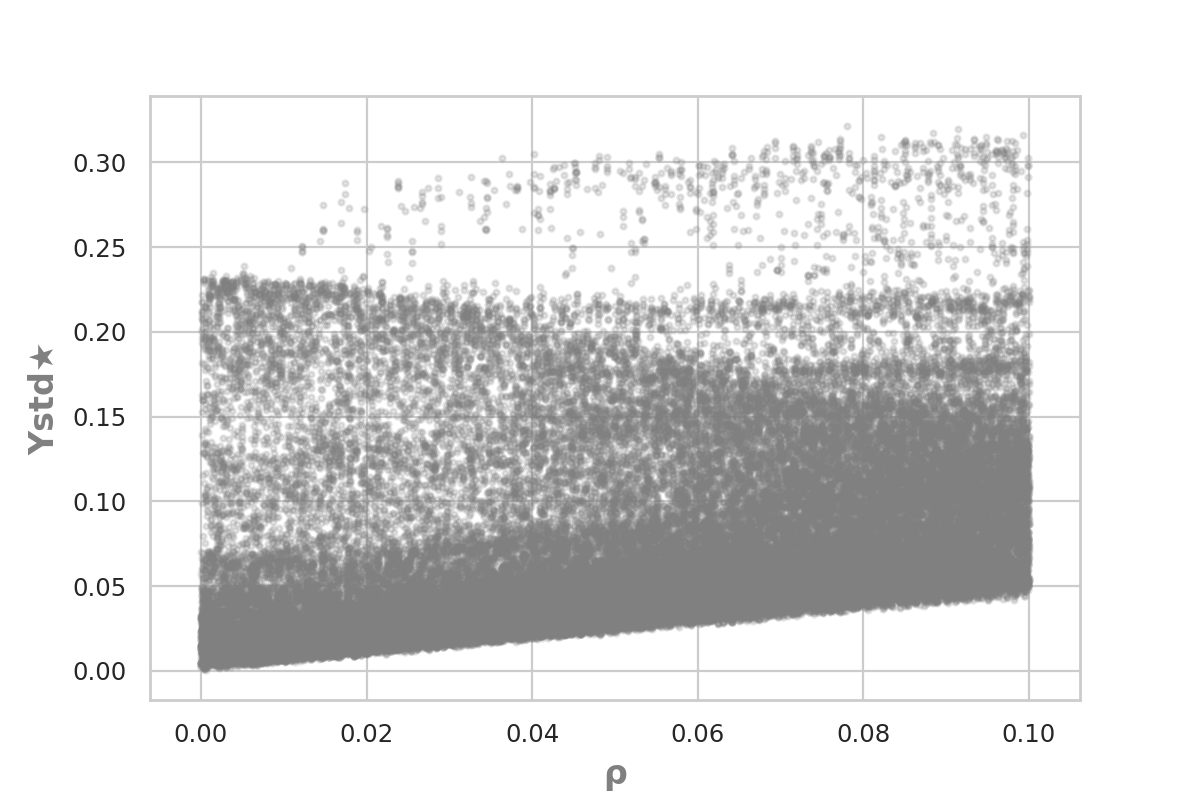
\includegraphics[width=\textwidth]{img/regressionYstd*rho.png}
 %      \caption{\(n\_issues = 1, \sigma = 0.02\) }
     \end{subfigure}
     \begin{subfigure}[b]{0.5\textwidth}
       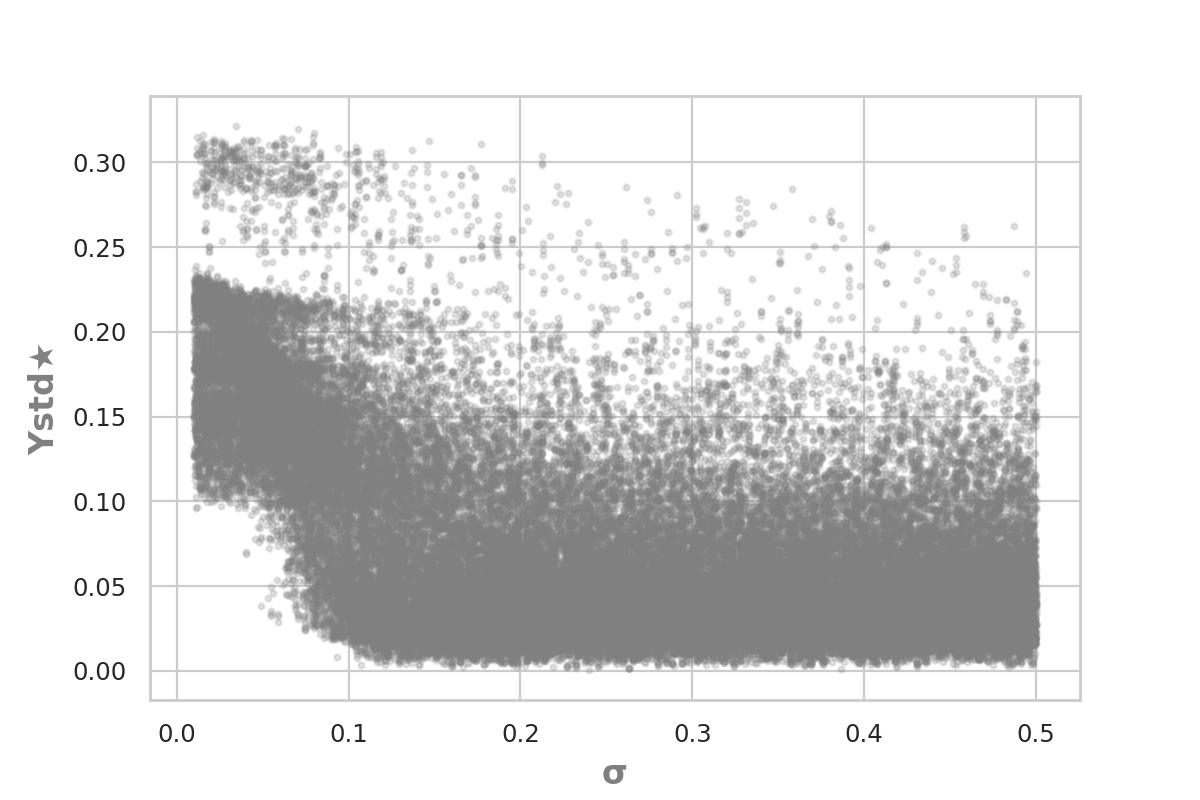
\includegraphics[width=\textwidth]{img/regressionYstd*sigma.png}
  %     \caption{\(n\_issues = 7, \sigma = 0.1\)}
     \end{subfigure}
     \caption{Scatterplots for the parameters with highest impact. Each dot corresponds to the result obtained in a single run.}
      \label{fig:scatters}
    \end{figure}



    The negative impact of \(\sigma\) in the population' opinion dispersion is
    expected: a higher \(\sigma\) means agents are easier to influence. As they
    are connected to all the other agents, the more uncertain they are, the more
    centralized the agents' mean opinions will tend to become. The plots also
    show that the exact value of \(\sigma\) seems to matter little above
    approximately 0.1. Therefore we restrict our following analysis to the
    \((0.0, 0.1 ] \) range. The effect of \(\rho\) is also expected: the bigger
    the noise, the more dispersed the final state of the system is. The number
    of issues $n$ seems to have little influence unless it is $n=1$. When there
    is only one issue, we see results where the opinions clearly move away to
    stronger polarizations, with (\(Ystd\)) around 0.3. Those cases are no
    longer observed as we have at least two issues.


    To better understand how parameters influence the results, we can look at
    typical behaviors for specific parameter values. We ran cases where we kept
    \(\rho = 0.05 \) ; \(N = 500\) ; \(p\_intran = 0.0\) fixed, for 500.000
    iterations, and test combinations of $\sigma = (0.02, 0.04, 0.1)$ and $ n =
    (1,5)$. The time series at Figure \ref{fig:tseries1} show the time evolution
    of the opinions of all $500$ agents. The graphics exhibit the typical
    behavior of the system for the case where agent $i$ estimates how $j$ is
    trustworthy by comparing $j$ opinion to its own average $(o_{i,k}$, that is
    the $p{***}$ case. Only results for $p{***}$ are show here because the time
    series for $p^*$ and $p{**}$ are visually almost identical to the ones in
    the figuress. We see that larger values \(\sigma\) lead the opinions towards
    the center: the bigger the \(\sigma\) is, the more agents will tend to move
    closer to the mean.



        \begin{figure}[H]
  \centering
    \begin{subfigure}[b]{0.33\textwidth}
      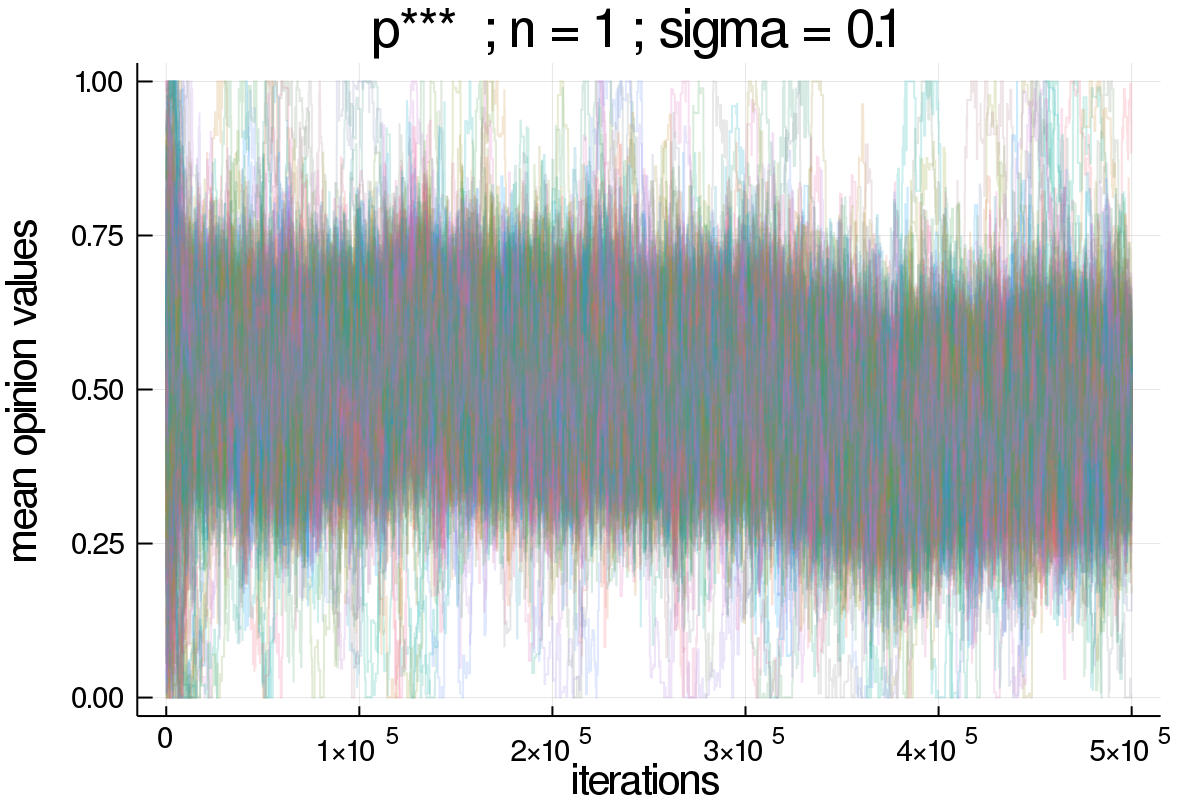
\includegraphics[width=\textwidth]{img/series/tseries1/Poodlcalculatep***n1-rho005-sigma01-00intransrandom.png}
      %\caption{\textcolor{red}{'ill fix thix}}
    \end{subfigure}
       \begin{subfigure}[b]{0.33\textwidth}
      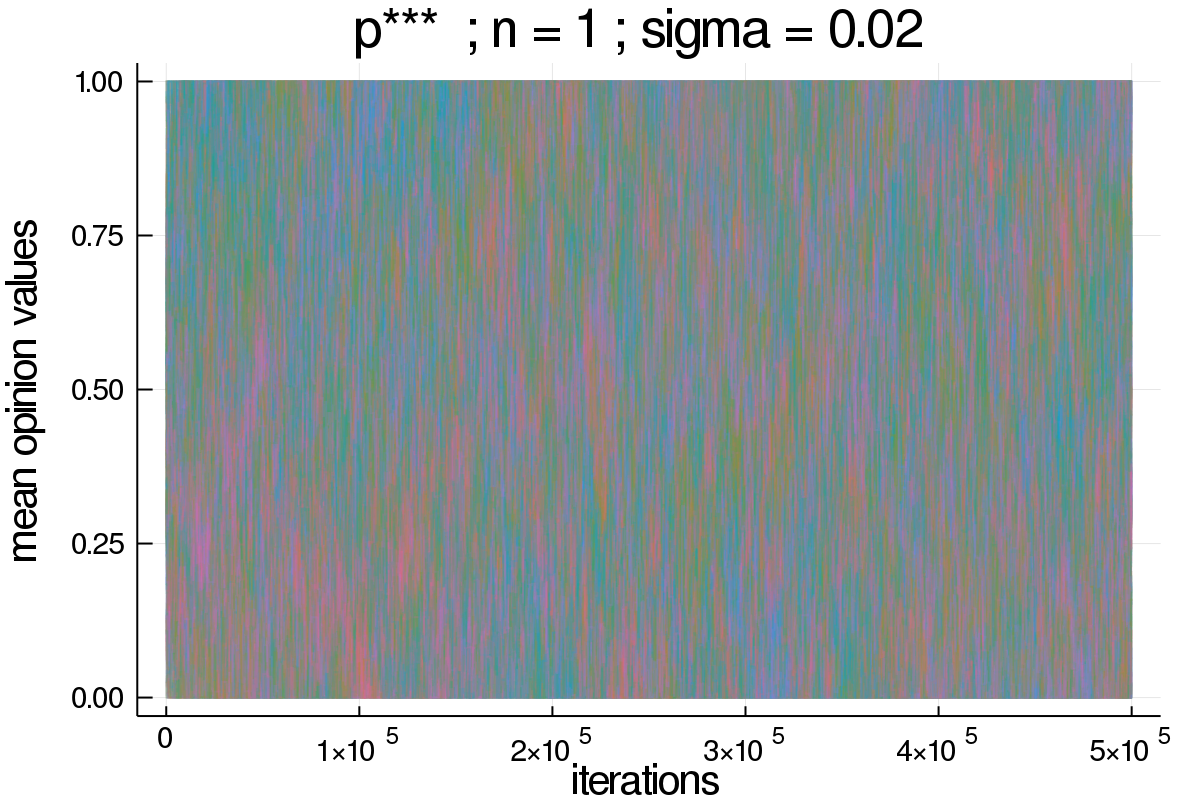
\includegraphics[width=\textwidth]{img/series/tseries1/Poodlcalculatep***n1-rho005-sigma002-00intransrandom.png}
 %      \caption{\(n\_issues = 1, \sigma = 0.02\) }
     \end{subfigure}
    \begin{subfigure}[b]{0.33\textwidth}
      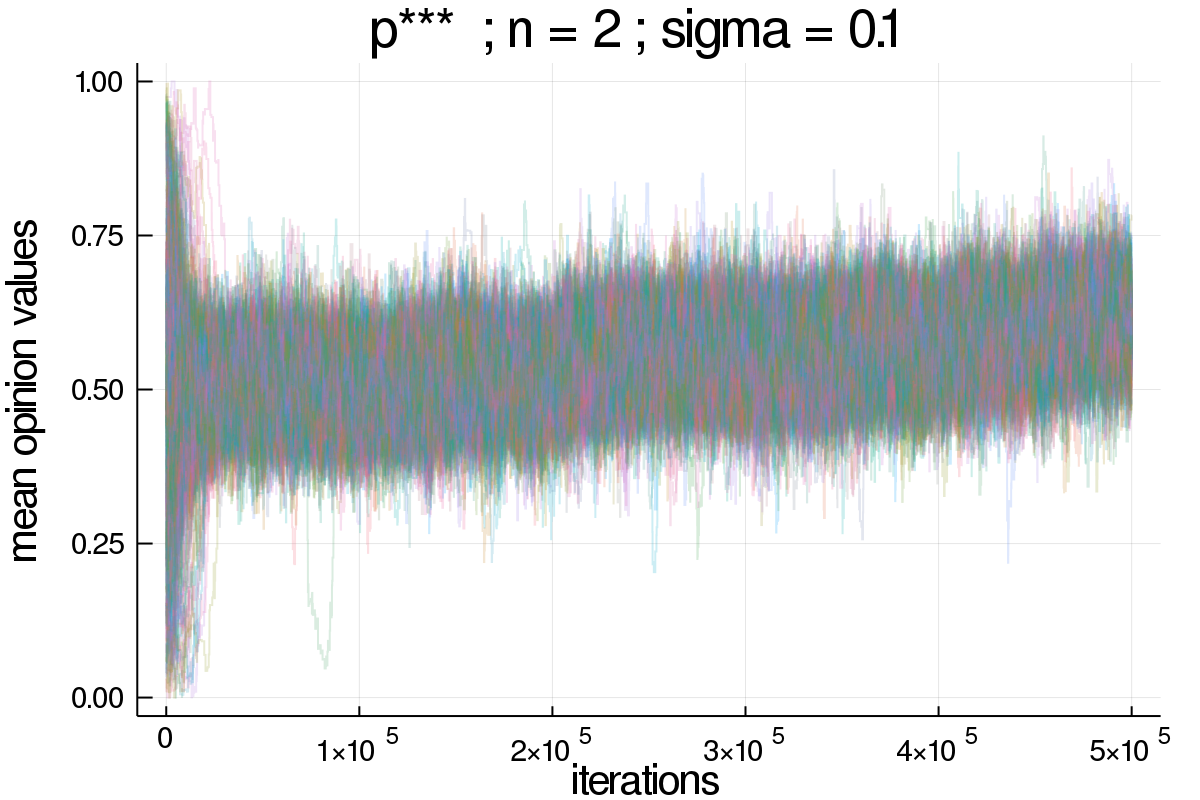
\includegraphics[width=\textwidth]{img/series/tseries1/Poodlcalculatep***n2-rho005-sigma01-00intransrandom.png}
 %      \caption{\(n\_issues = 1, \sigma = 0.02\) }
    \end{subfigure}
     \begin{subfigure}[b]{0.33\textwidth}
       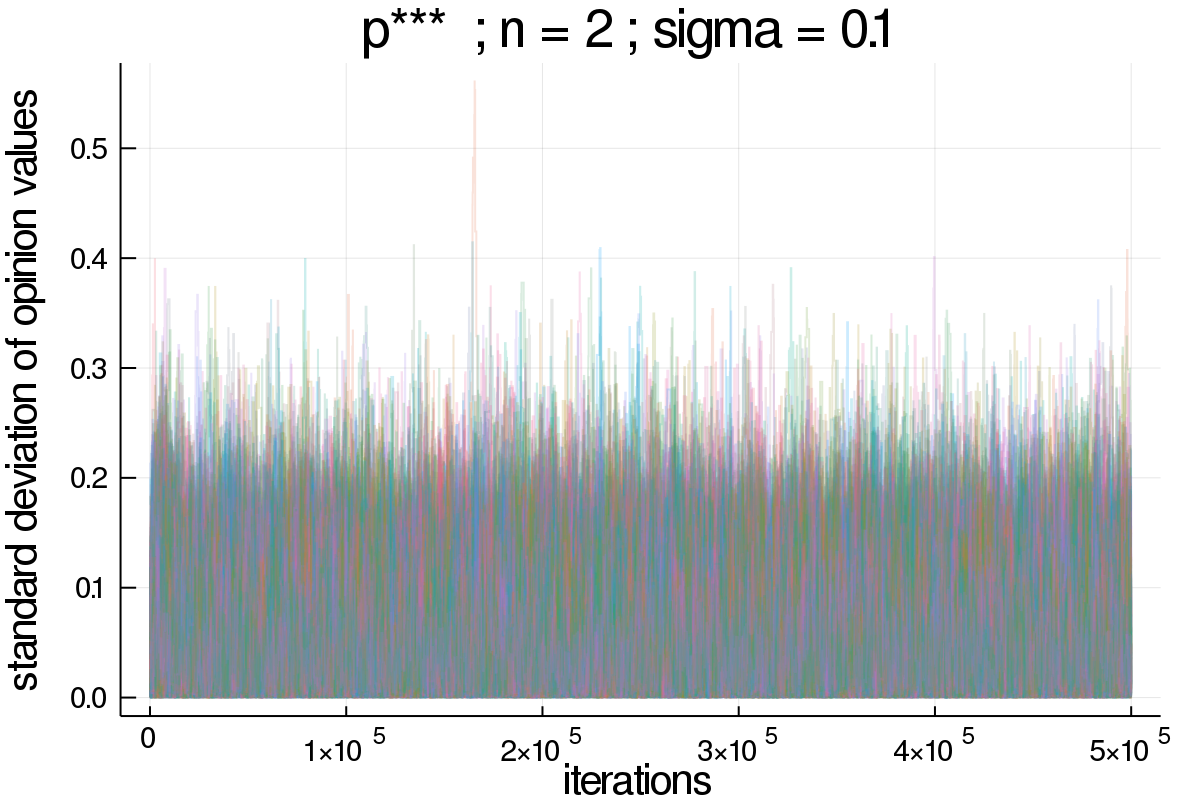
\includegraphics[width=\textwidth]{img/series/tseries1/Poodlcalculatep***n2-rho005-sigma01-00intransrandom-std.png}
     \end{subfigure}
     
              \begin{subfigure}[b]{0.33\textwidth}
      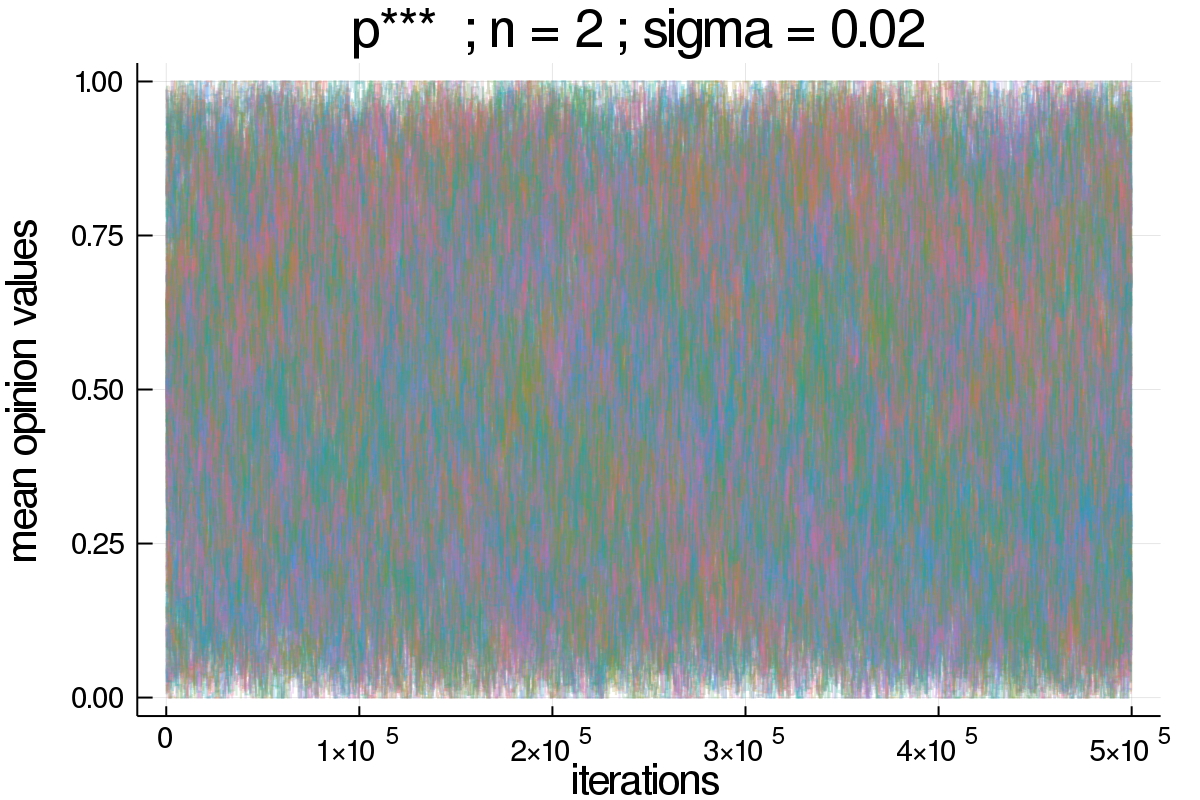
\includegraphics[width=\textwidth]{img/series/tseries1/Poodlcalculatep***n2-rho005-sigma002-00intransrandom.png}
 %      \caption{\(n\_issues = 1, \sigma = 0.02\) }
     \end{subfigure}
    \begin{subfigure}[b]{0.33\textwidth}
      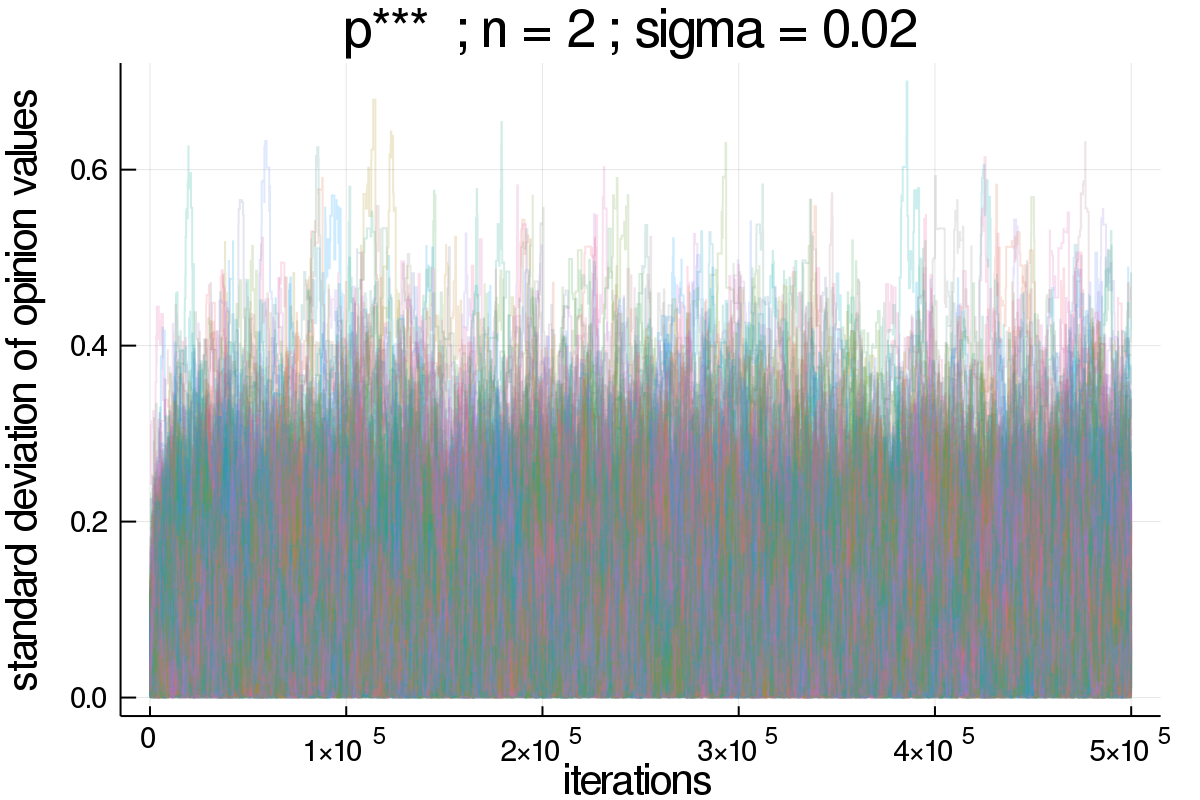
\includegraphics[width=\textwidth]{img/series/tseries1/Poodlcalculatep***n2-rho005-sigma002-00intransrandom-std.png}
%     \caption{\(n\_issues = 7, \sigma = 0.1\)}
     \end{subfigure}
     \caption{Time series for the parameterization: \(\rho = 0.05, N = 500,
       p\_intran = 0.0, n  = 1 \) or  $2$}
      \label{fig:tseries1}
    \end{figure}




    Figure \ref{fig:tseries2} shows similar time evolution series for $n=5$
    issues. Here, even for small values of $\sigma$ we observe the opinions tend
    to avoid the more extreme values. That seems to be an artifact of initial
    random draws. While it is easy to draw the most extreme values with only one
    draw, for $n=5$, as we are close to the end of the range, no values outside
    that range are possible. So, the most extreme values require that, at the
    start, agents should have all their five issues drawn as extreme. As that is
    rare, those few that do start there tend to be attracted to still extreme
    positions, but a little less so. However, there also seems to be an actual
    tendency towards more central opinions. That can be oberved as $\sigma$
    increases and the tendency to consensus around a central position becomes
    even stronger than in the $n=1$ case.


    
    \begin{figure}[H]
      \centering
      \begin{subfigure}[b]{0.3\textwidth}
        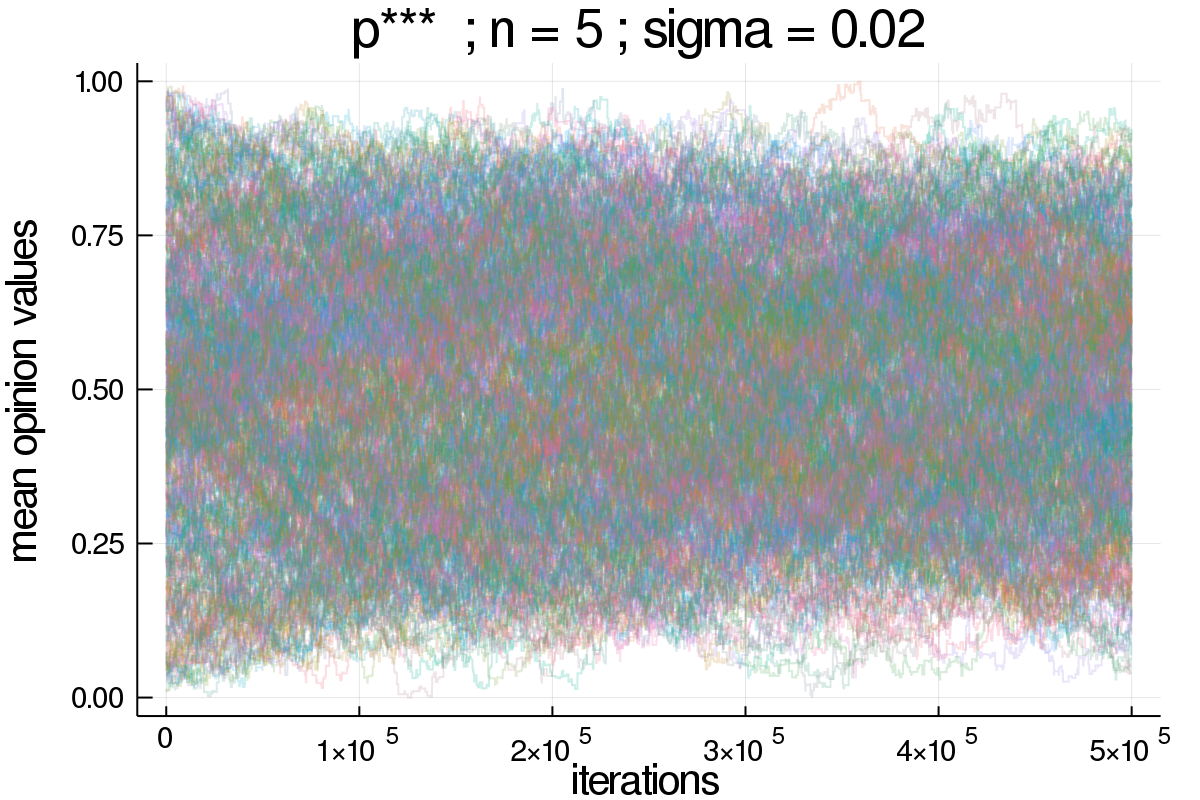
\includegraphics[width=\textwidth]{img/series/tseries2/Poodlcalculatep***n5-rho005-sigma002-00intransrandom.png}
        % \caption{\textcolor{red}{'ill fix thix}}
      \end{subfigure}
      \begin{subfigure}[b]{0.3\textwidth}
        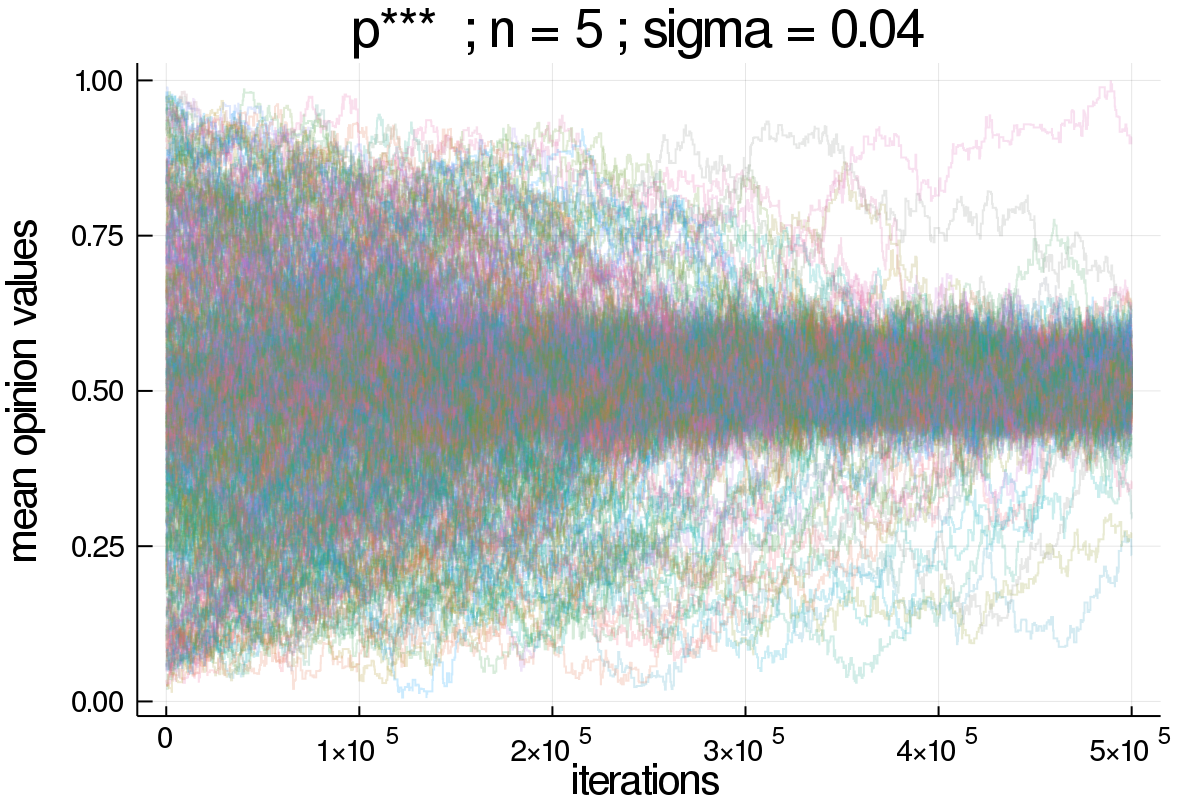
\includegraphics[width=\textwidth]{img/series/tseries2/Poodlcalculatep***n5-rho005-sigma004-00intransrandom.png}
        % \caption{\(n\_issues = 1, \sigma = 0.02\) }
      \end{subfigure}
      \begin{subfigure}[b]{0.3\textwidth}
        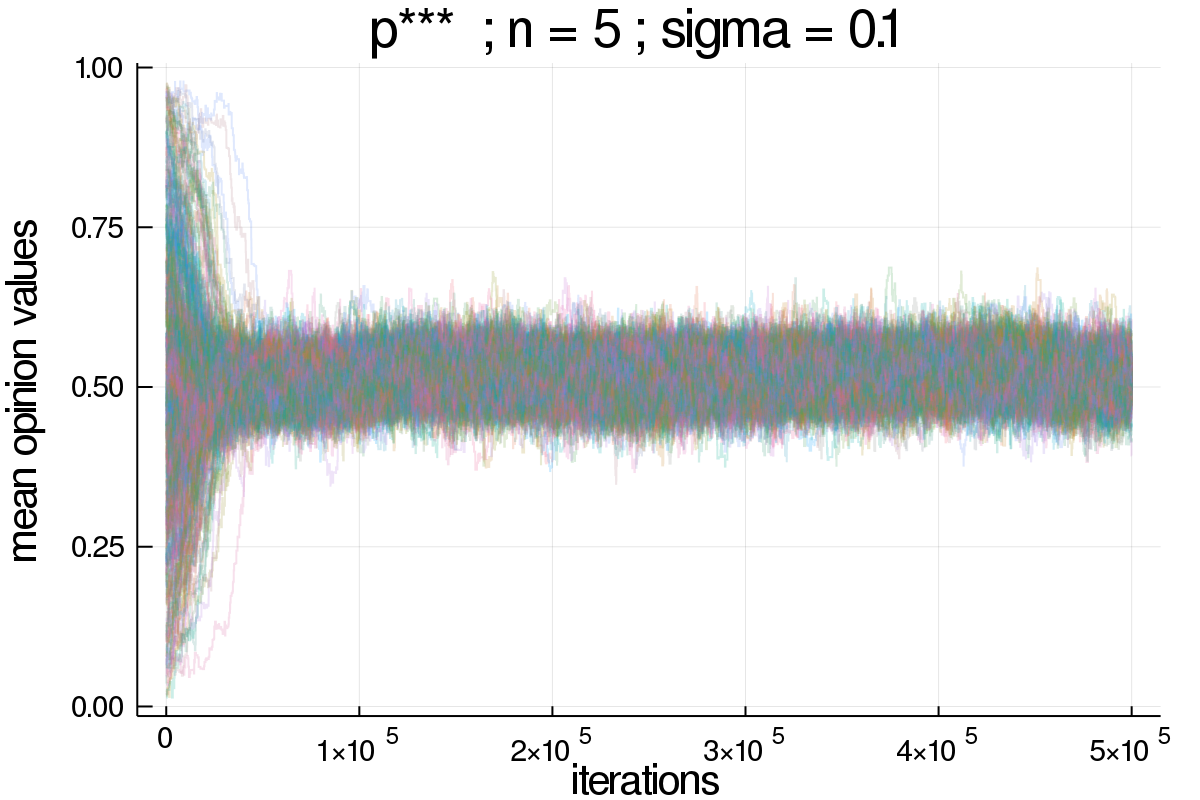
\includegraphics[width=\textwidth]{img/series/tseries2/Poodlcalculatep***n5-rho005-sigma01-00intransrandom.png}
        % \caption{\(n\_issues = 7, \sigma = 0.1\)}
      \end{subfigure}

           \begin{subfigure}[b]{0.3\textwidth}
        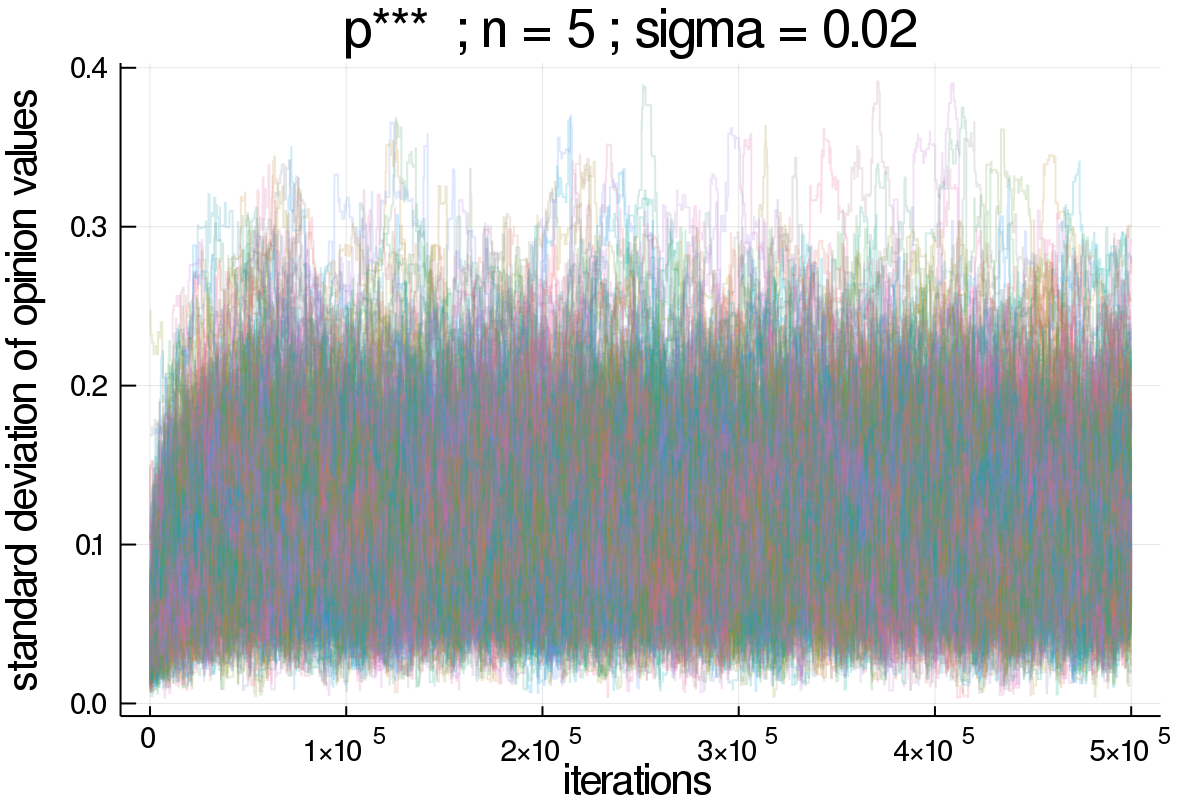
\includegraphics[width=\textwidth]{img/series/tseries2/Poodlcalculatep***n5-rho005-sigma002-00intransrandom-std.png}
        % \caption{\textcolor{red}{'ill fix thix}}
      \end{subfigure}
      \begin{subfigure}[b]{0.3\textwidth}
        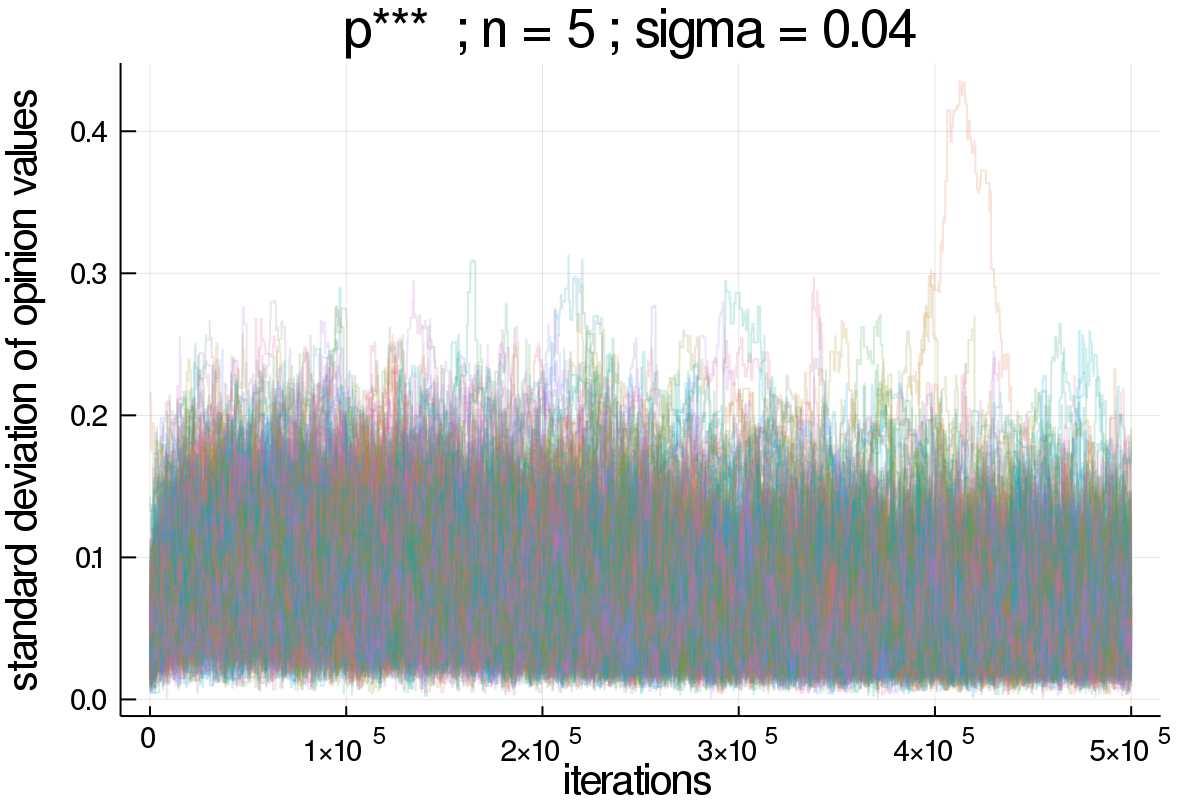
\includegraphics[width=\textwidth]{img/series/tseries2/Poodlcalculatep***n5-rho005-sigma004-00intransrandom-std.png}
        % \caption{\(n\_issues = 1, \sigma = 0.02\) }
      \end{subfigure}
      \begin{subfigure}[b]{0.3\textwidth}
        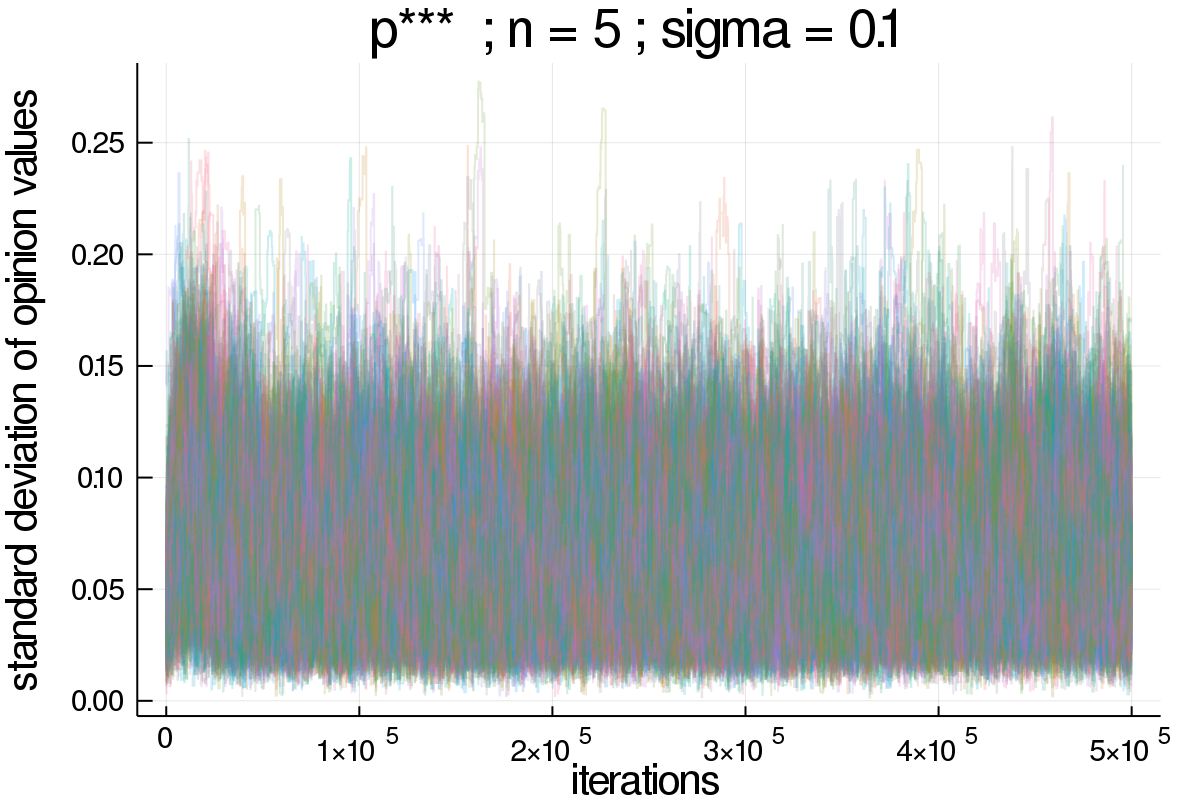
\includegraphics[width=\textwidth]{img/series/tseries2/Poodlcalculatep***n5-rho005-sigma01-00intransrandom-std.png}
        % \caption{\(n\_issues = 7, \sigma = 0.1\)}
      \end{subfigure}
      \caption{Time series for the parameterization: \(\rho = 0.05, N = 500,
        p\_intran = 0.0\)}
            \label{fig:tseries2}
          \end{figure}
          
    The reason for that is : we're measuring the mean opinion values (\(x_i\))
    and \(\rho\) changes a single \(o_i\) at each iteration which means that a
    higher \(n\) implies a lesser impact of \(\rho\) on the mean opinion of the
    agent, since she will have \(n-1\) other opinions stabilizing her mean
    opinion at a point in the opinion spectrum. As \(\sigma\) is the parameter
    that dominates the model update rule it interacts with \(n\), which enforces
    \(\sigma\) effect whenever we test higher \(n\)s. This effect holds even
    when we raise \(\rho\) together with \(n\). Let's use the same
    parameterization as the last plot but with a new \(\rho\) such that \(\rho_2
    = \sqrt{n} * \rho_1 = \sqrt{10} * 0.05\). The interaction between \(n\) and
    \(\sigma\) still happens, with bigger \(n\) stabilizing the noise effect and
    contributing to the centralizing effect of \(\sigma\), even though a bigger
    \(\rho\) leads to more noise around the mean. 

    
    \begin{figure}[H]
      \centering
      \begin{subfigure}[b]{0.45\textwidth}
      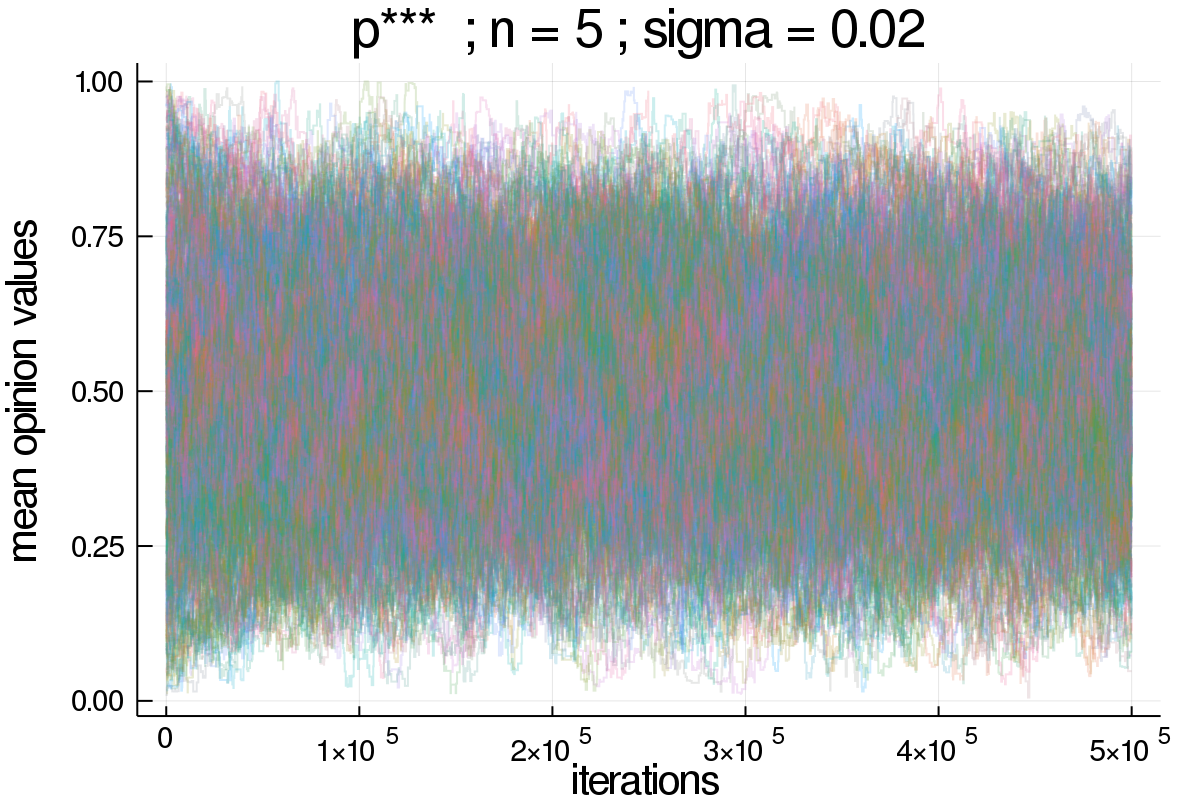
\includegraphics[width=0.9\textwidth]{img/series/tseries3/Poodlcalculatep***n5-rho01118033988749895-sigma002-00intransrandom.png}
    \end{subfigure}
          \begin{subfigure}[b]{0.45\textwidth}
      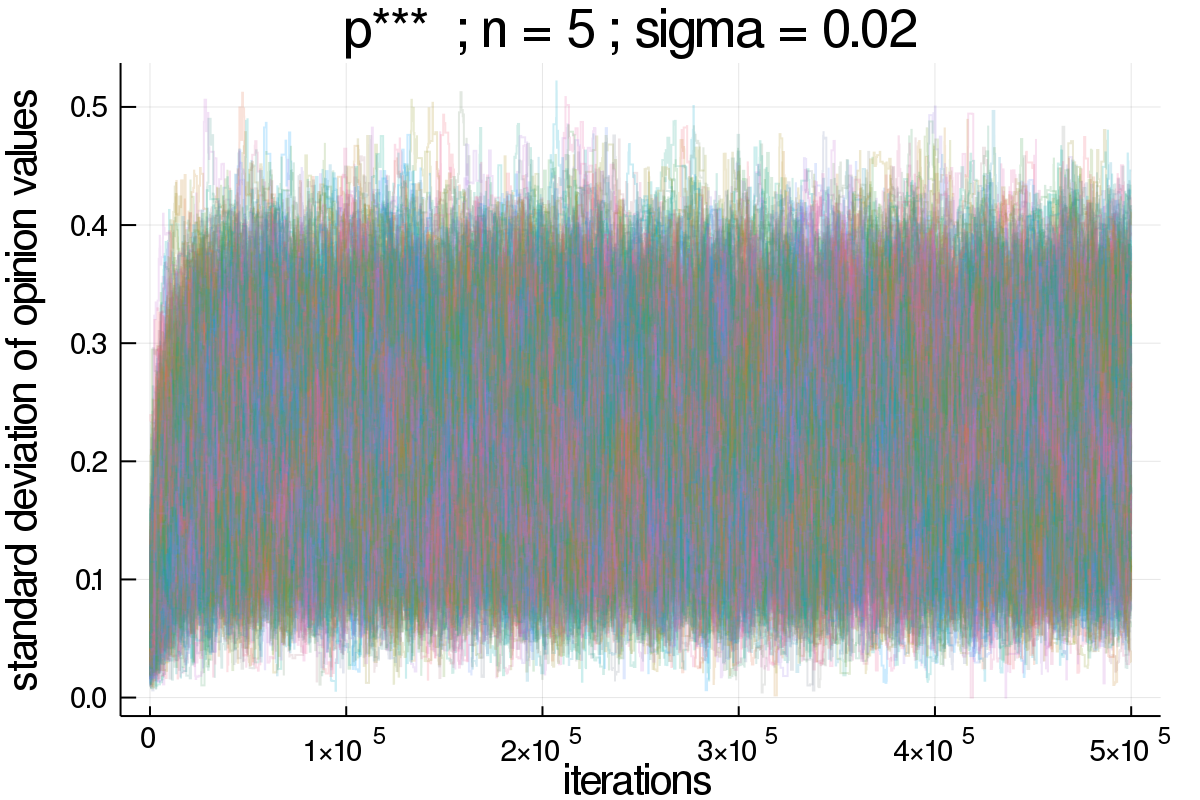
\includegraphics[width=0.9\textwidth]{img/series/tseries3/Poodlcalculatep***n5-rho01118033988749895-sigma002-00intransrandom-std.png}
    \end{subfigure}
    \begin{subfigure}[b]{0.45\textwidth}
      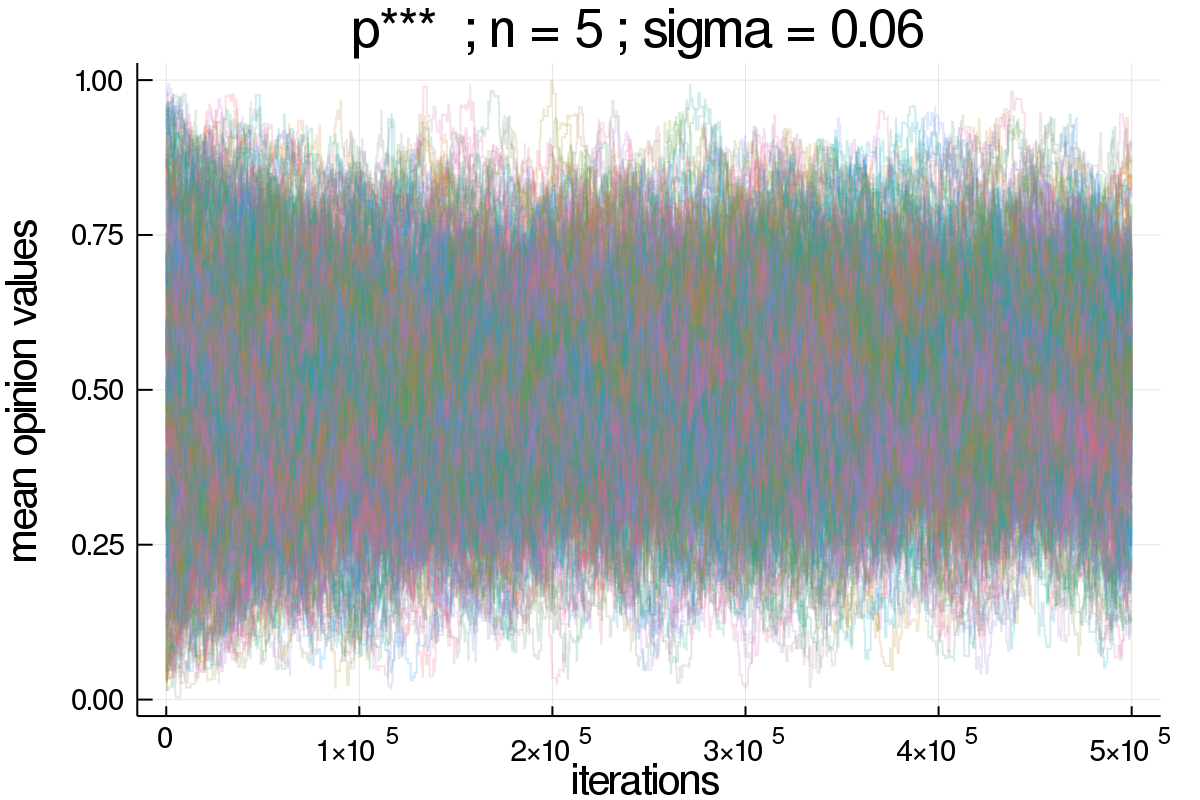
\includegraphics[width=0.9\textwidth]{img/series/tseries3/Poodlcalculatep***n5-rho01118033988749895-sigma006-00intransrandom.png}
    \end{subfigure}
    \begin{subfigure}[b]{0.45\textwidth}
      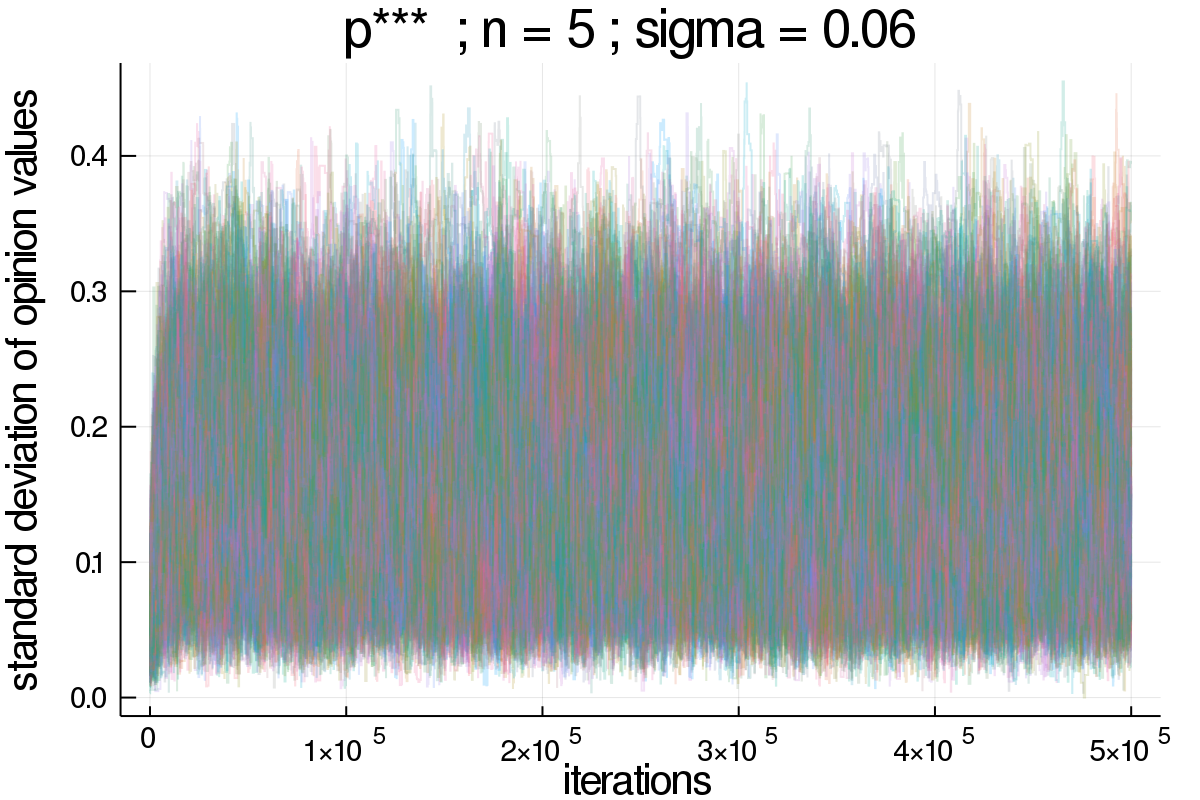
\includegraphics[width=0.9\textwidth]{img/series/tseries3/Poodlcalculatep***n5-rho01118033988749895-sigma006-00intransrandom-std.png}
    \end{subfigure}
      \begin{subfigure}[b]{0.45\textwidth}
      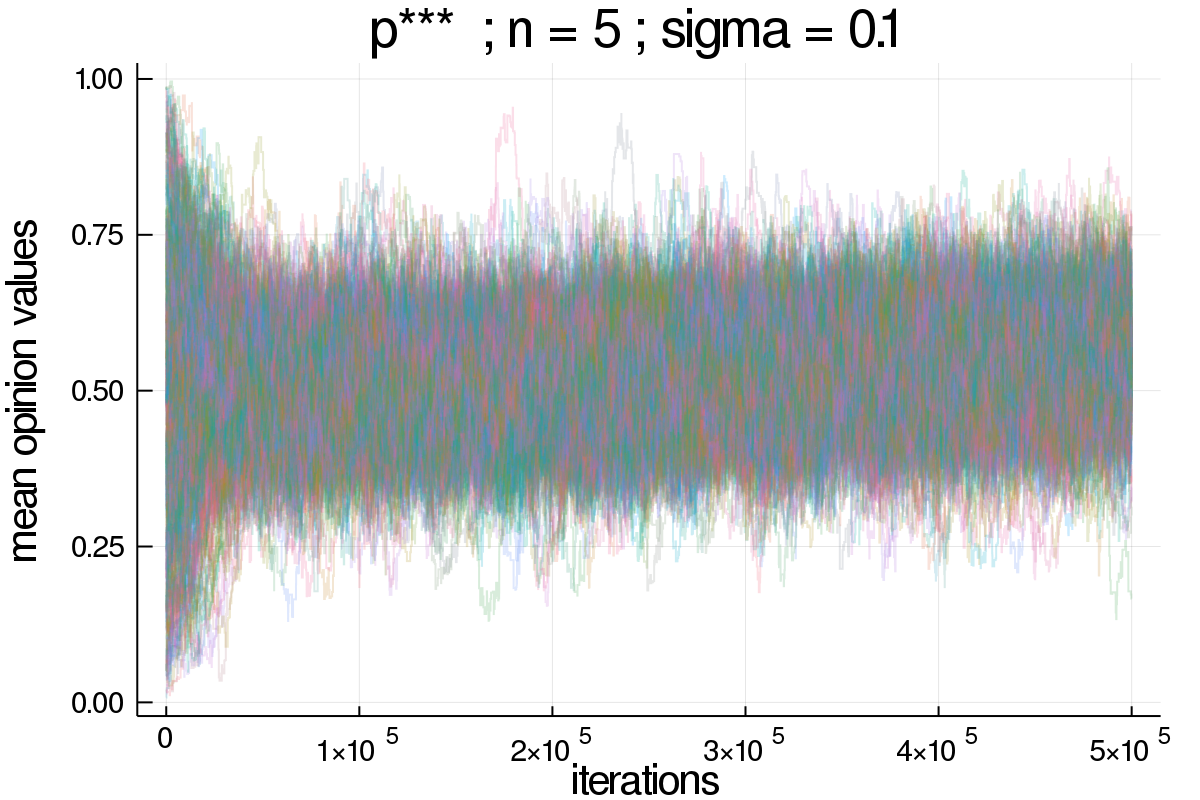
\includegraphics[width=0.9\textwidth]{img/series/tseries3/Poodlcalculatep***n5-rho01118033988749895-sigma01-00intransrandom.png}
    \end{subfigure}
  \begin{subfigure}[b]{0.45\textwidth}
      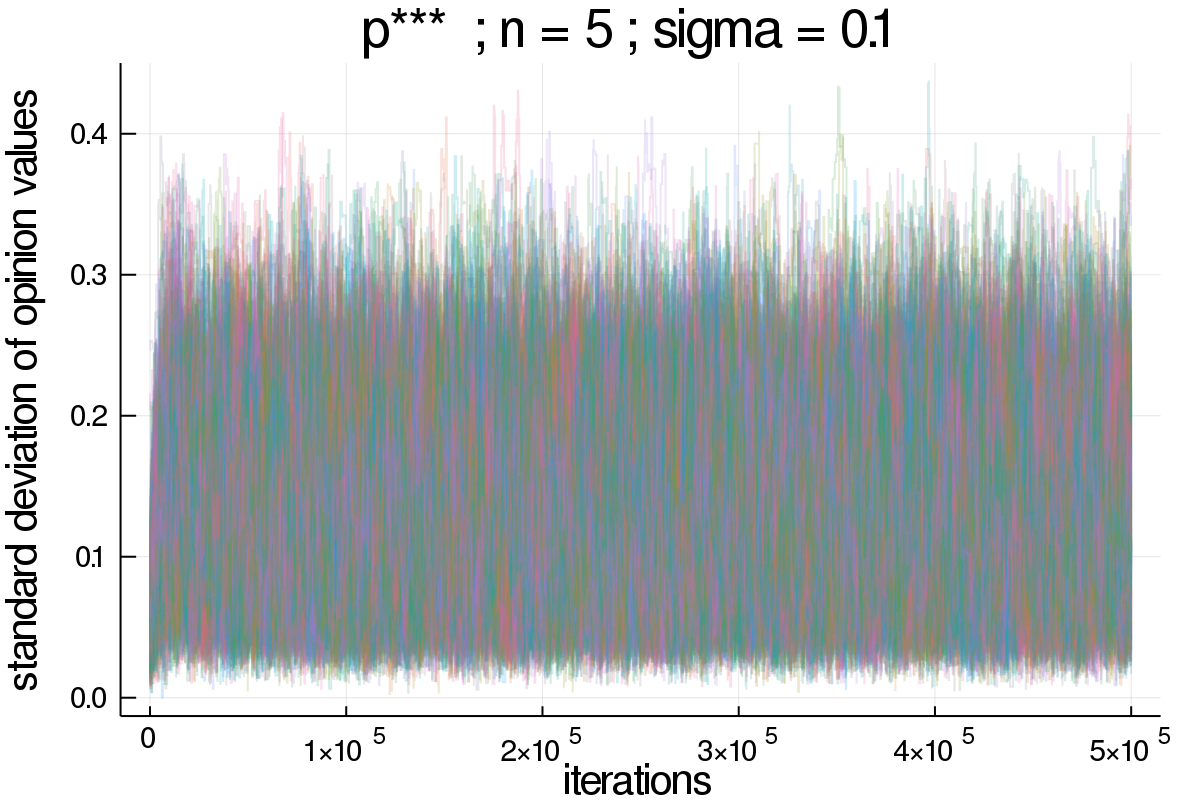
\includegraphics[width=0.9\textwidth]{img/series/tseries3/Poodlcalculatep***n5-rho01118033988749895-sigma01-00intransrandom-std.png}
      \end{subfigure}
    
      \caption{Time series for the parameterization: \(\rho \approx 0.12, N =
        500, p\_intran = 0.0 \)}
      \label{fig:tseries3}
    \end{figure}

    Heretofore we've tested parameterizations with noise, but what happens if we
    lower \(\rho\) to a value close to zero, such as 1e-5? The first difference is
    that the population mean opinion values converge to certain values. In
    parameter combinations in which \(\sigma = 0.1\) the tendency is convergence
    to values close to 0.5. An interesting distinction between the cases in this
    parameterization is that \(p^{**}\) and \(p^{***}\) always converge to 0.5,
    independently of the number of issues. Alternatively, in the \(p^{*}\) case
    this happens when \(n=1\), but when we have \(n=5\) or \(10\) there are
    other values of convergence, more as we increase \(n\), even though the
    centralizing tendency remains.
    \begin{figure}[H]
      \centering
      \begin{subfigure}[b]{0.45\textwidth}
        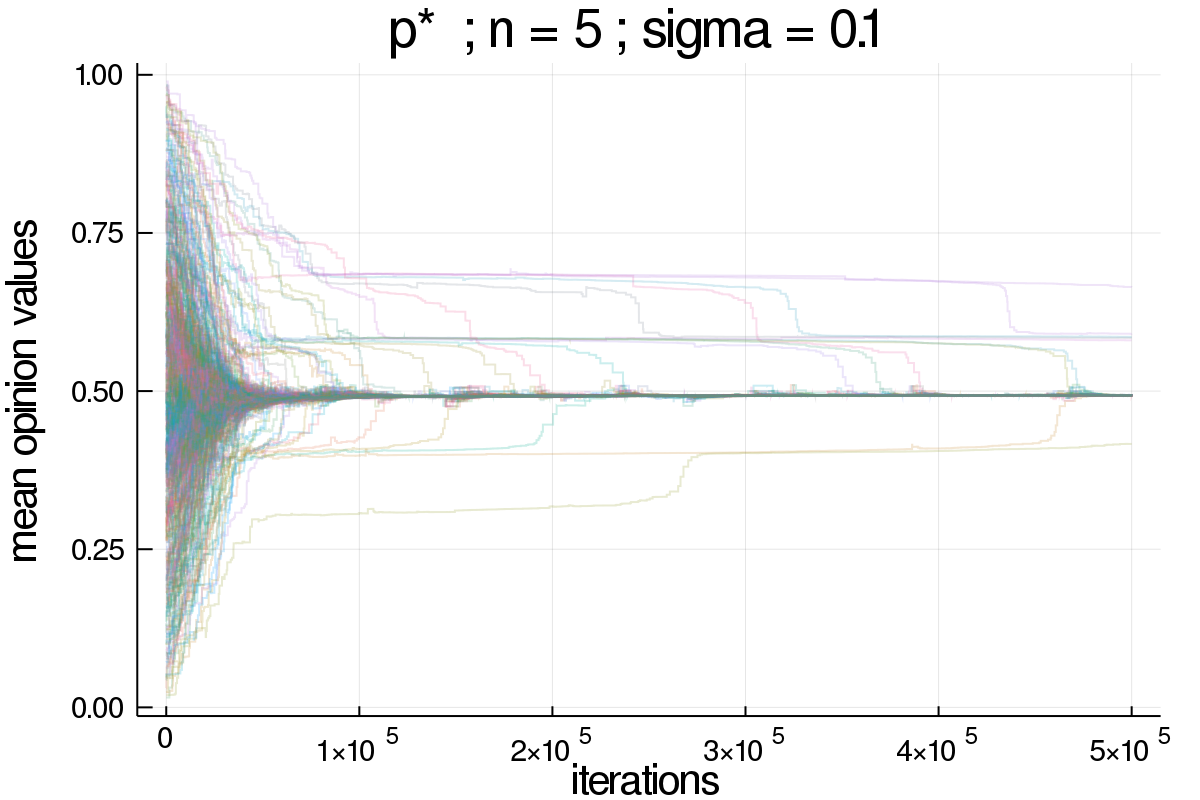
\includegraphics[width=\textwidth]{img/series/tseries4/Poodlcalculatep*n5-rho10e-5-sigma01-00intransrandom.png}
        % \caption{\textcolor{red}{'ill fix thix}}
      \end{subfigure}
      \begin{subfigure}[b]{0.45\textwidth}
        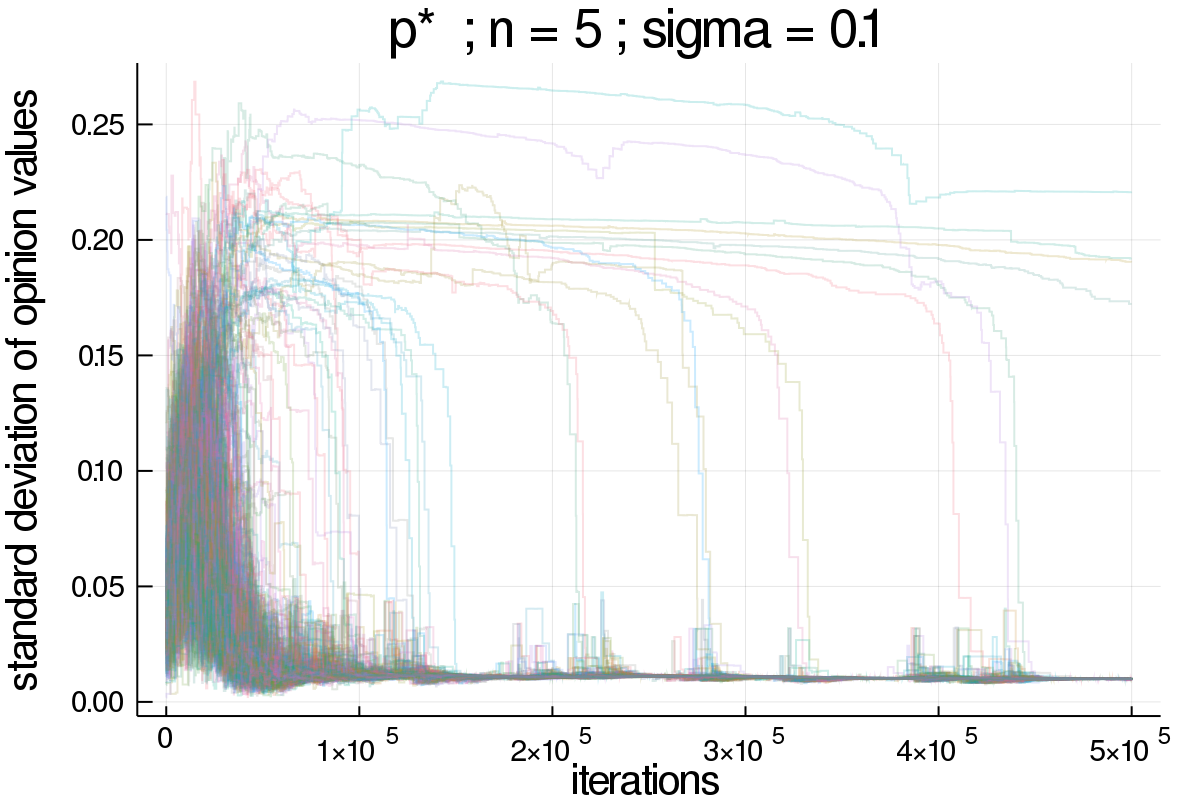
\includegraphics[width=\textwidth]{img/series/tseries4/Poodlcalculatep*n5-rho10e-5-sigma01-00intransrandom-std.png}
        % \caption{\textcolor{red}{'ill fix thix}}
      \end{subfigure}
      \begin{subfigure}[b]{0.45\textwidth}
        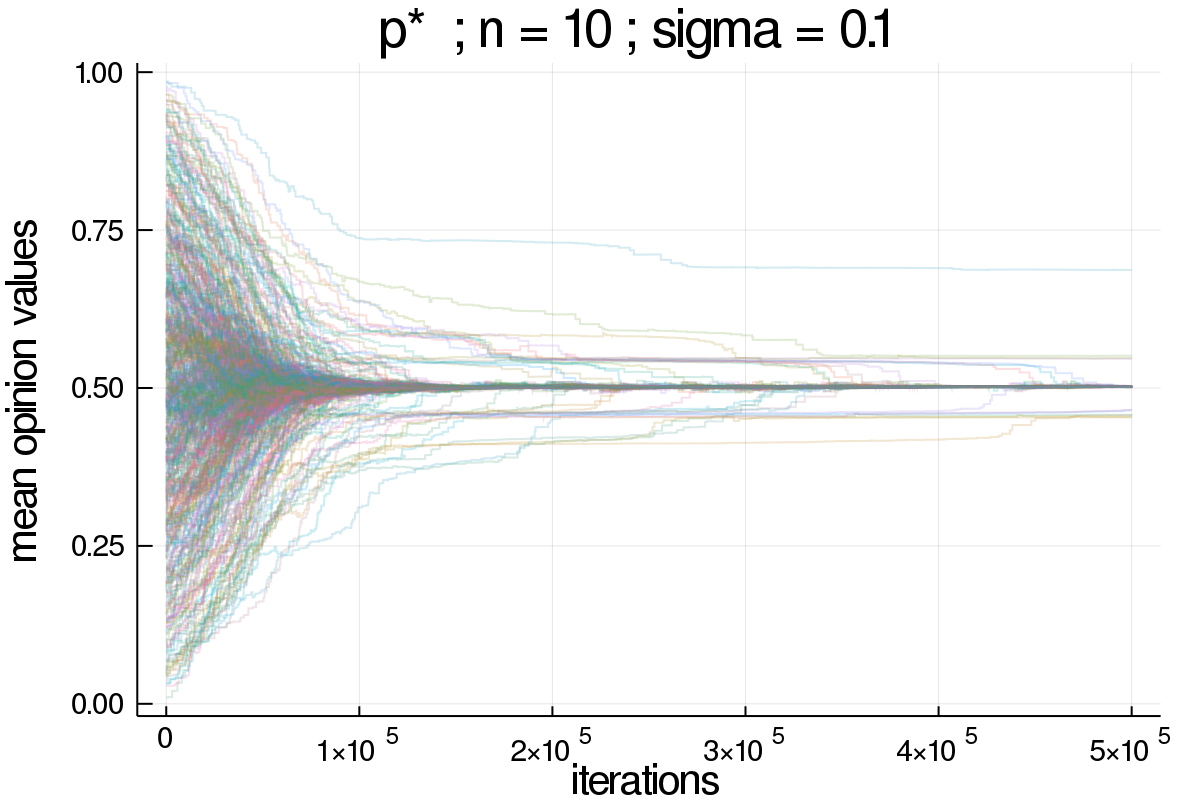
\includegraphics[width=\textwidth]{img/series/tseries4/Poodlcalculatep*n10-rho10e-5-sigma01-00intransrandom.png}
        % \caption{\(n\_issues = 1, \sigma = 0.02\) }
      \end{subfigure}
      \begin{subfigure}[b]{0.45\textwidth}
        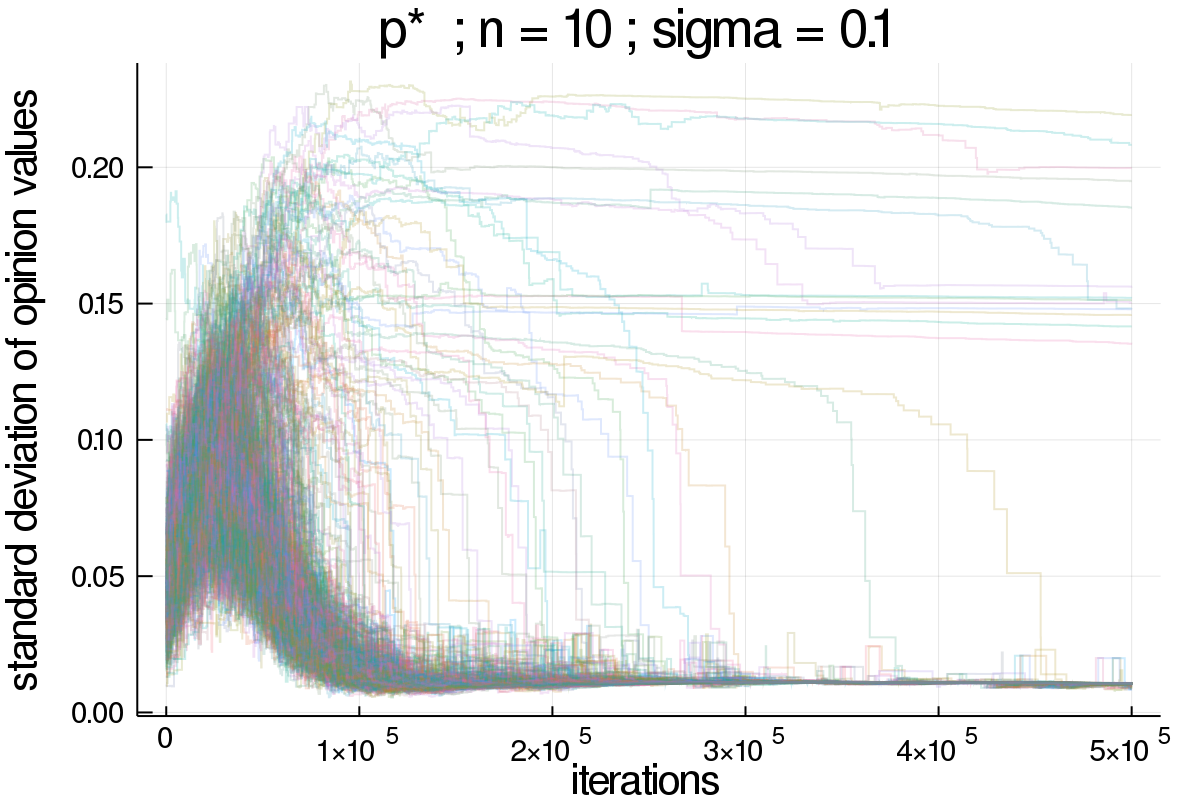
\includegraphics[width=\textwidth]{img/series/tseries4/Poodlcalculatep*n10-rho10e-5-sigma01-00intransrandom-std.png}
        % \caption{\(n\_issues = 1, \sigma = 0.02\) }
      \end{subfigure}
      \begin{subfigure}[b]{0.45\textwidth}
        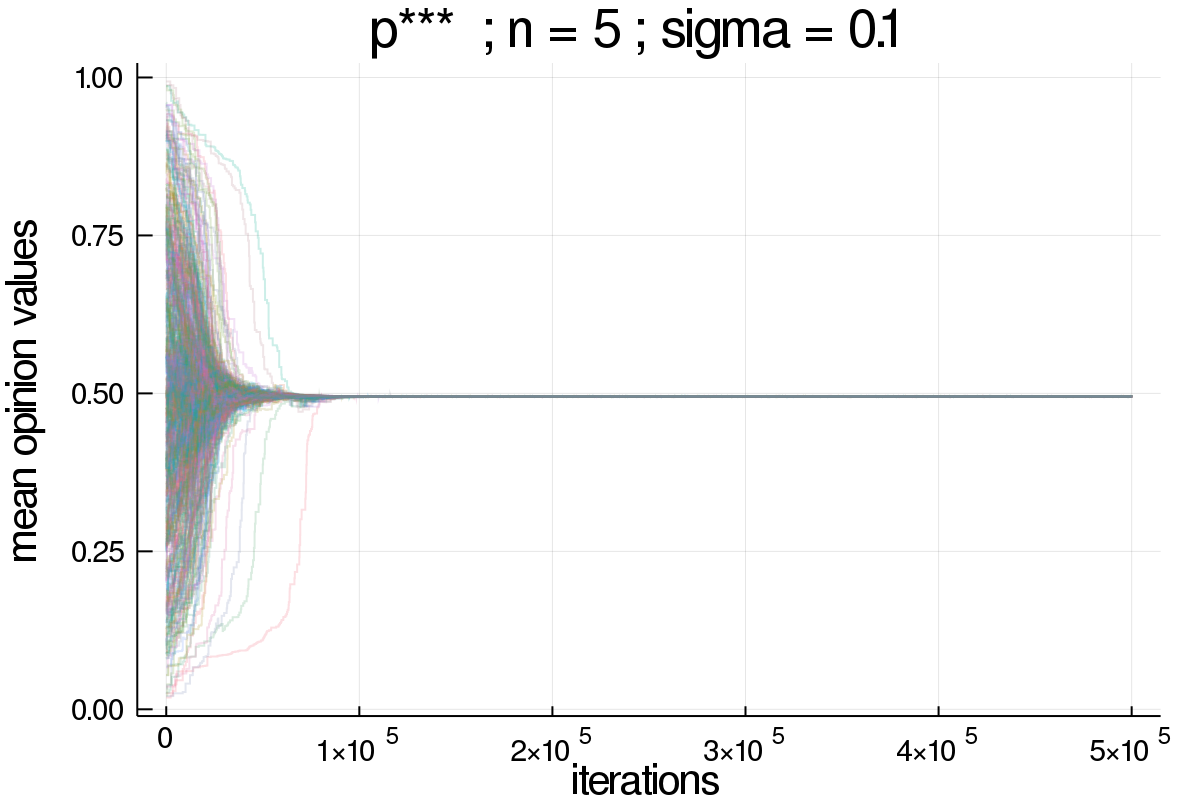
\includegraphics[width=\textwidth]{img/series/tseries4/Poodlcalculatep***n5-rho10e-5-sigma01-00intransrandom.png}
        % \caption{\(n\_issues = 7, \sigma = 0.1\)}
      \end{subfigure}
      \begin{subfigure}[b]{0.45\textwidth}
        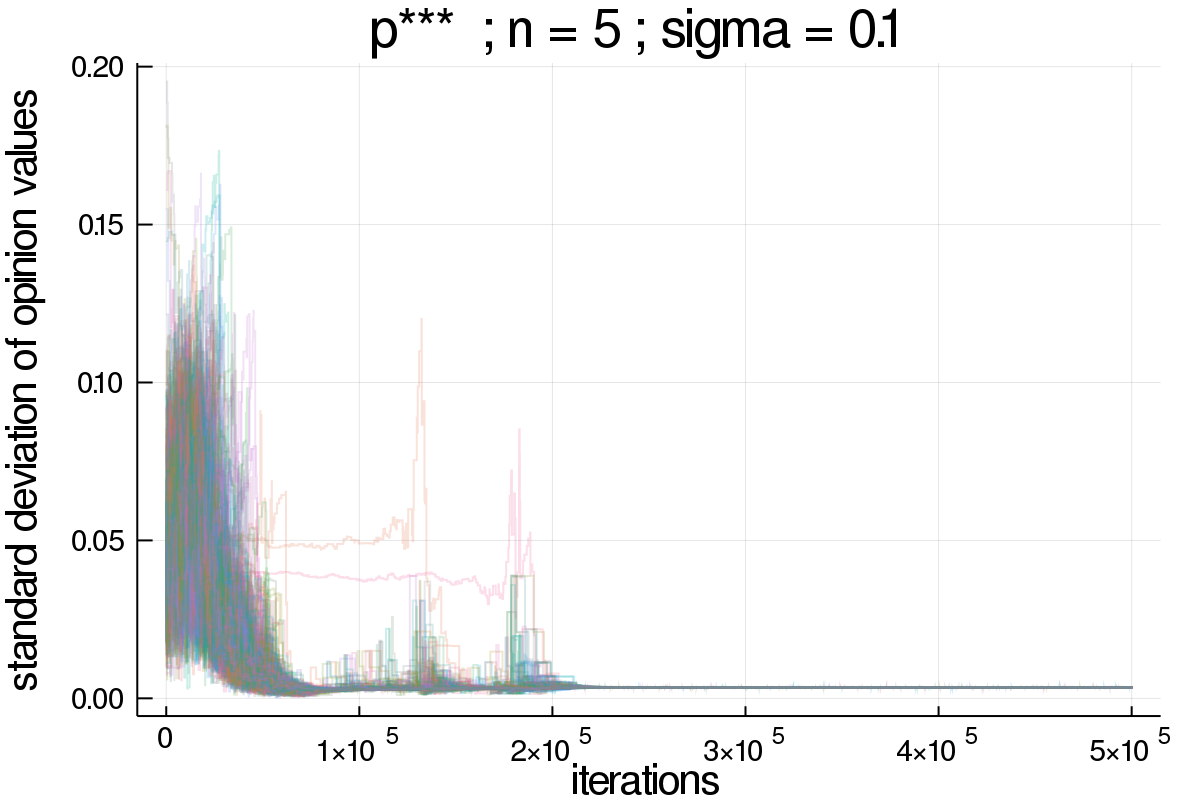
\includegraphics[width=\textwidth]{img/series/tseries4/Poodlcalculatep***n5-rho10e-5-sigma01-00intransrandom-std.png}
        % \caption{\(n\_issues = 7, \sigma = 0.1\)}
      \end{subfigure}
            \begin{subfigure}[b]{0.45\textwidth}
        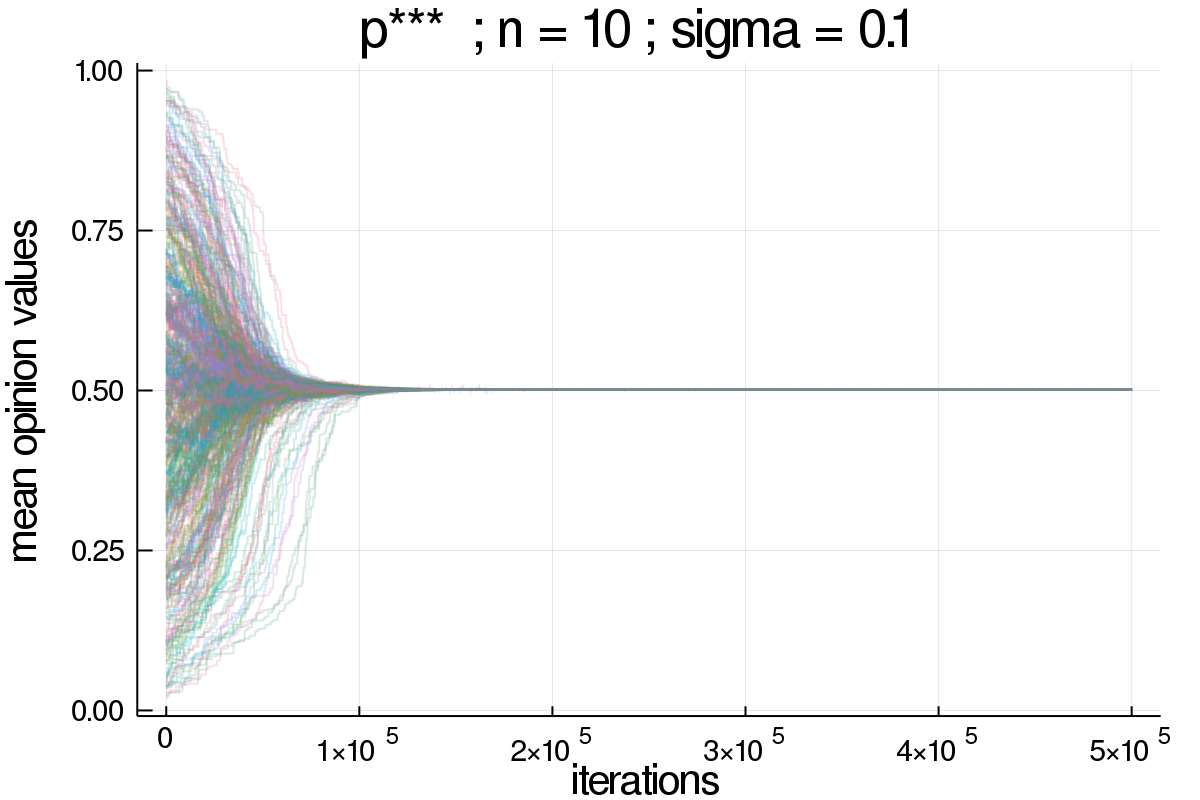
\includegraphics[width=\textwidth]{img/series/tseries4/Poodlcalculatep***n10-rho10e-5-sigma01-00intransrandom.png}
        % \caption{\(n\_issues = 7, \sigma = 0.1\)}
      \end{subfigure}
      \begin{subfigure}[b]{0.45\textwidth}
        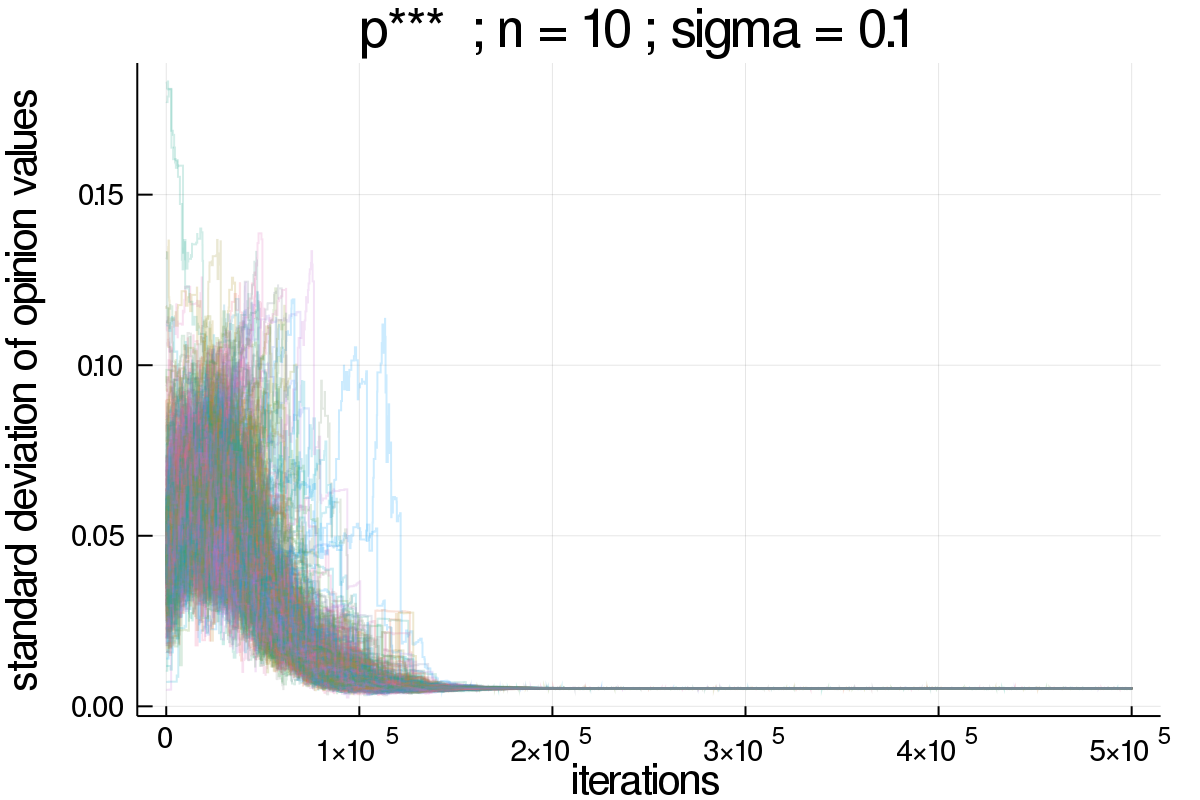
\includegraphics[width=\textwidth]{img/series/tseries4/Poodlcalculatep***n10-rho10e-5-sigma01-00intransrandom-std.png}
        % \caption{\(n\_issues = 7, \sigma = 0.1\)}
      \end{subfigure}
      \caption{Time series for the parameterization: \(\rho = 1e-5, N =
        500, p\_intran = 0.0 \)}
      \label{fig:tseries4}
    \end{figure}
    In the parameterization in which \(\sigma\) is of intermediate value (for
    our range), such as \(0.02\) or \(0.04\), we observe another difference
    between cases: \(p^{*}\) has more convergence values than \(p^{**}\) and
    \(p^{***}\). Figure \ref{fig:tseries5} illustrates this system behavior:

    \begin{figure}[H]
      \centering
      \begin{subfigure}[b]{0.45\textwidth}
        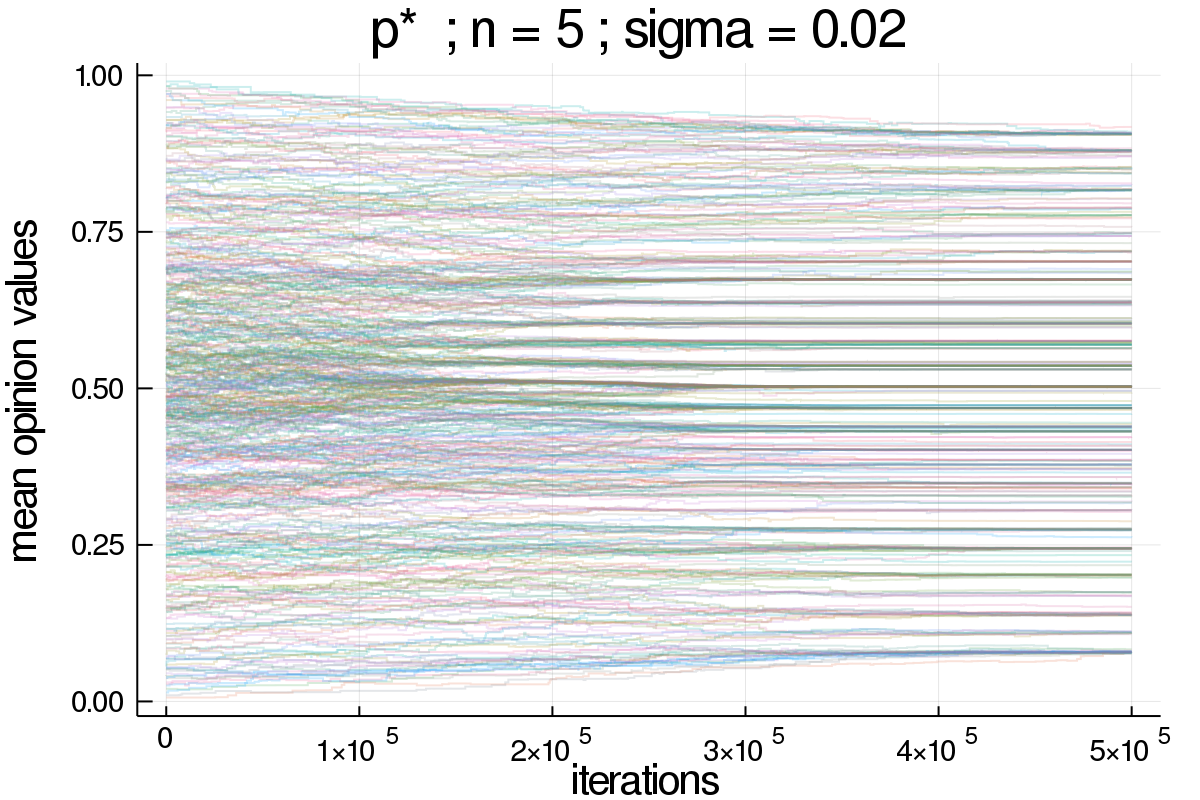
\includegraphics[width=\textwidth]{img/series/tseries5/Poodlcalculatep*n5-rho10e-5-sigma002-00intransrandom.png}
        % \caption{\textcolor{red}{'ill fix thix}}
      \end{subfigure}
      \begin{subfigure}[b]{0.45\textwidth}
        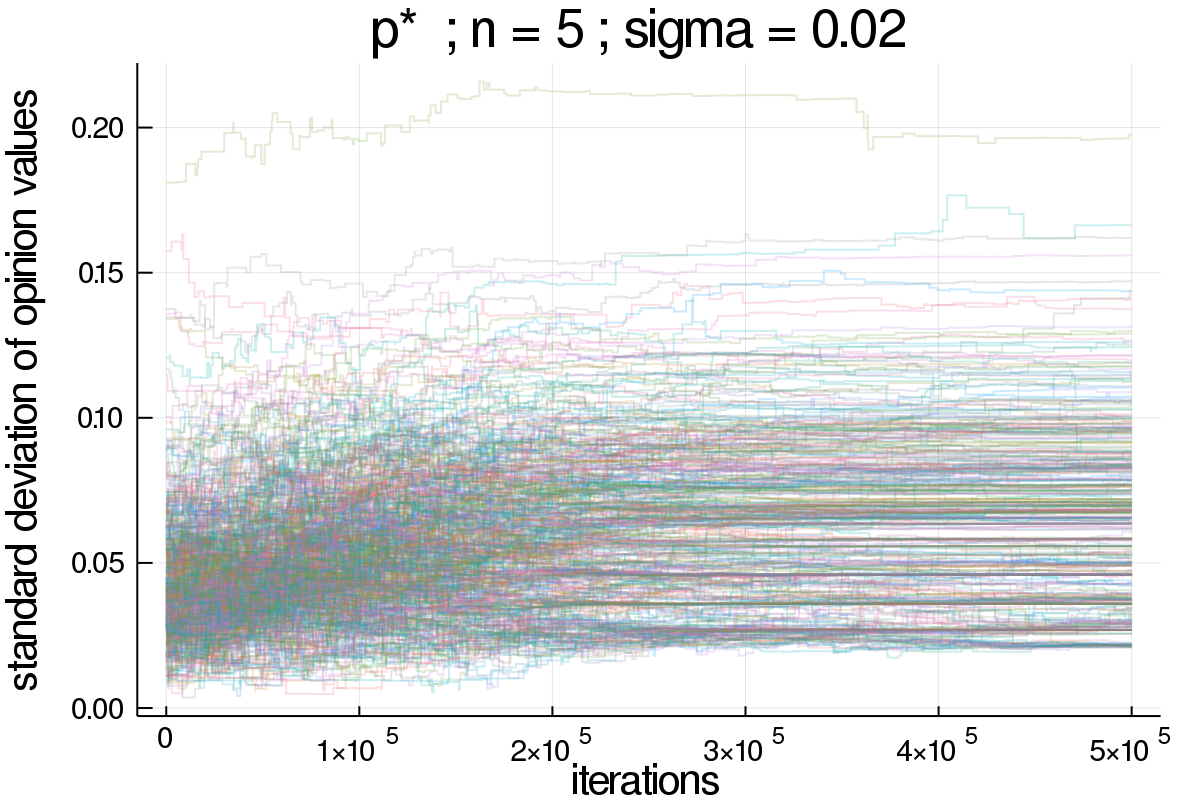
\includegraphics[width=\textwidth]{img/series/tseries5/Poodlcalculatep*n5-rho10e-5-sigma002-00intransrandom-std.png}
        % \caption{\textcolor{red}{'ill fix thix}}
        \end{subfigure}
      \begin{subfigure}[b]{0.45\textwidth}
        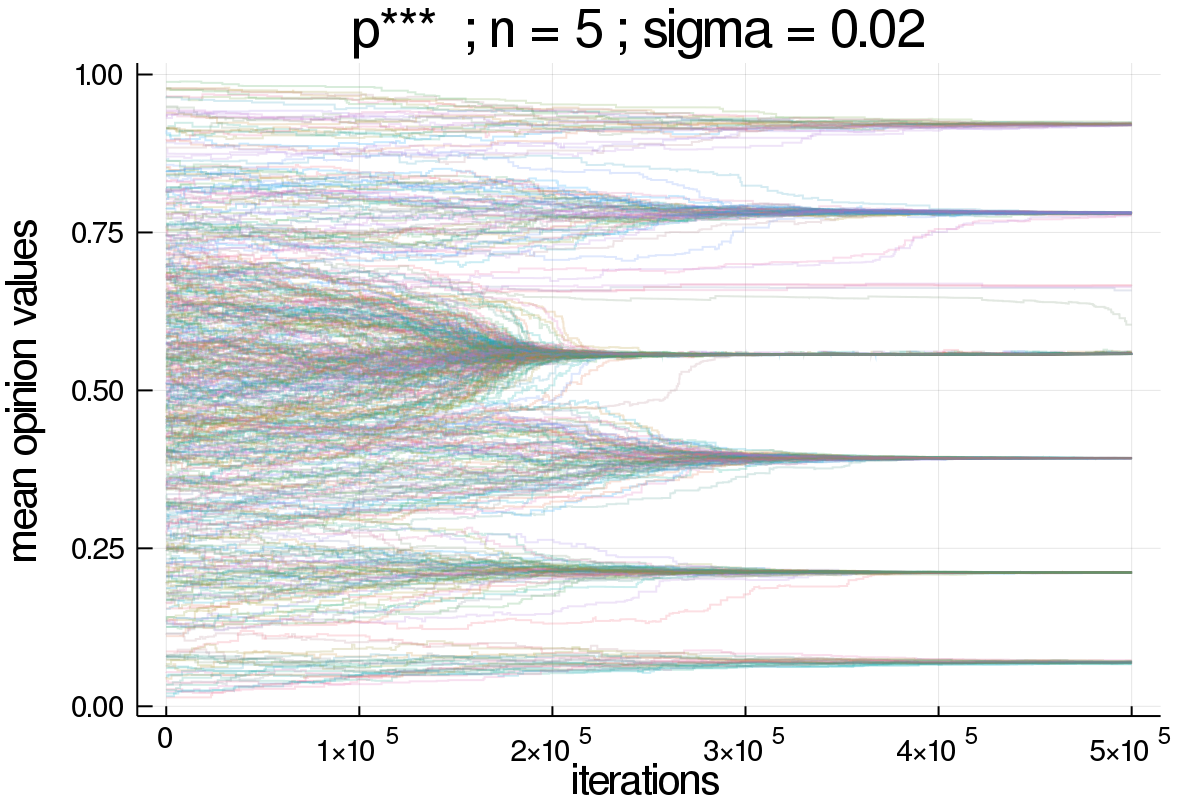
\includegraphics[width=\textwidth]{img/series/tseries5/Poodlcalculatep***n5-rho10e-5-sigma002-00intransrandom.png}
        % \caption{\(n\_issues = 1, \sigma = 0.02\) }
      \end{subfigure}
      \begin{subfigure}[b]{0.45\textwidth}
        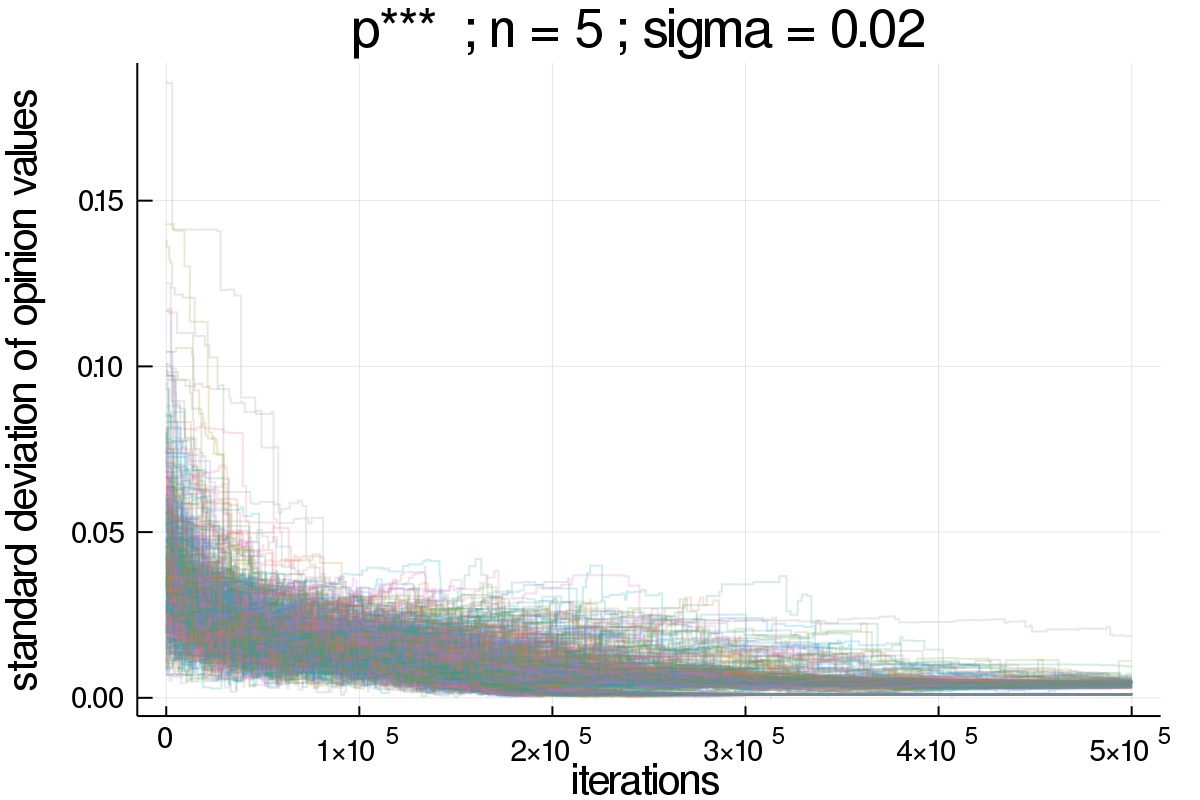
\includegraphics[width=\textwidth]{img/series/tseries5/Poodlcalculatep***n5-rho10e-5-sigma002-00intransrandom-std.png}
        % \caption{\(n\_issues = 1, \sigma = 0.02\) }
      \end{subfigure}
      \caption{Time series for the parameterization: \(\rho = 1e-5, N =
        500, p\_intran = 0.0 \)}      
  \label{fig:tseries5}
    \end{figure}

    The reason for that lies in the \(\Delta\) of each case: in the \(p^{**}\)
    and \(p^{***}\) cases the update rules make use of mean opinion values which
    facilitates the opinion convergence. The \(p^{*}\) update rule works with
    single issue opinions which opens the possibility that there is little
    influence between agents given their ideological distance at the issue.
    
    Another impact of the number of issues, as shown in Figure
    \ref{fig:tseries6}, is that a higher \(n\) leads to a longer time for the
    convergence to certain values. The reason is that we're only changing one
    opinion by iteration, so naturally a higher \(n\) means the agents will take
    longer to be influenced. The relationship here is roughly linear such that
    the plot the region at \(5 \times 10^5\) iterations when \(n = 10\) is very
    similar to the corresponding region at \(0.5 \times 10^5\) when \(n = 1\).
    
    \begin{figure}[H]
      \centering
      
      \begin{subfigure}[b]{0.49\textwidth}
        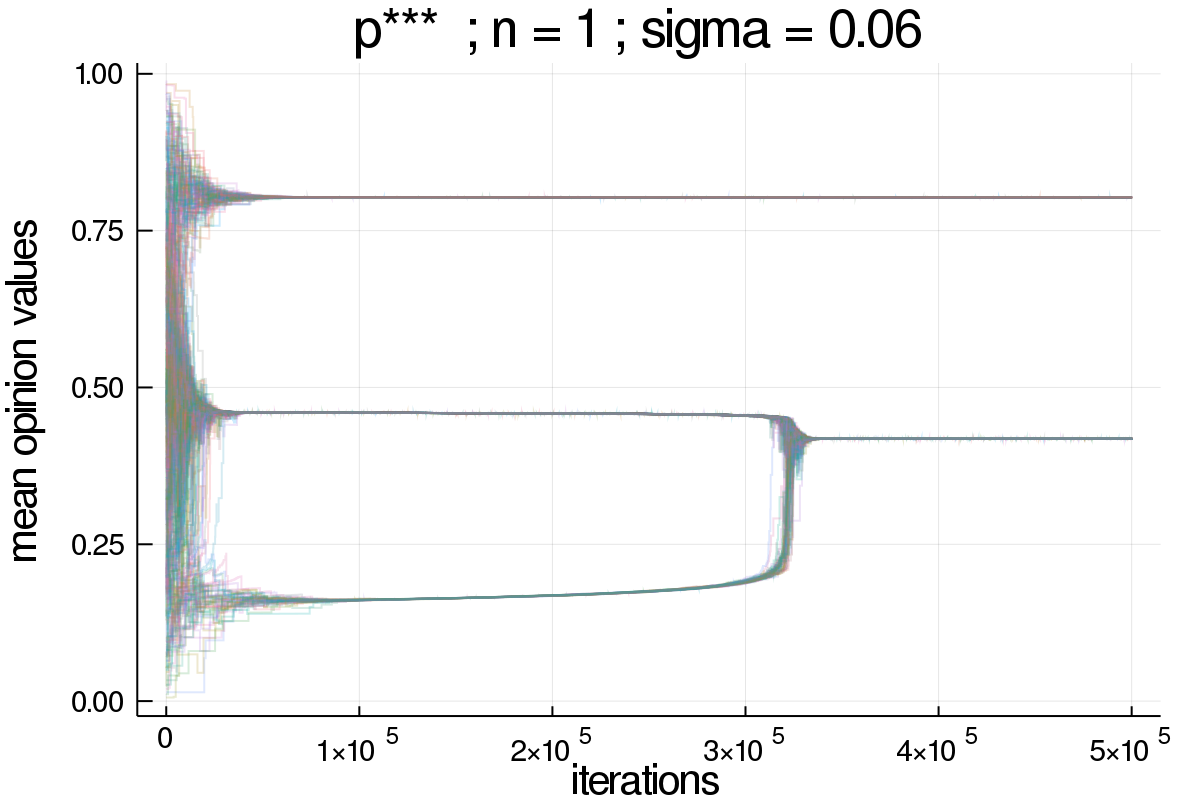
\includegraphics[width=\textwidth]{img/series/tseries6/Poodlcalculatep***n1-rho10e-5-sigma006-00intransrandom.png}
        % \caption{\textcolor{red}{'ill fix thix}}
      \end{subfigure}
      
      \begin{subfigure}[b]{0.49\textwidth}
        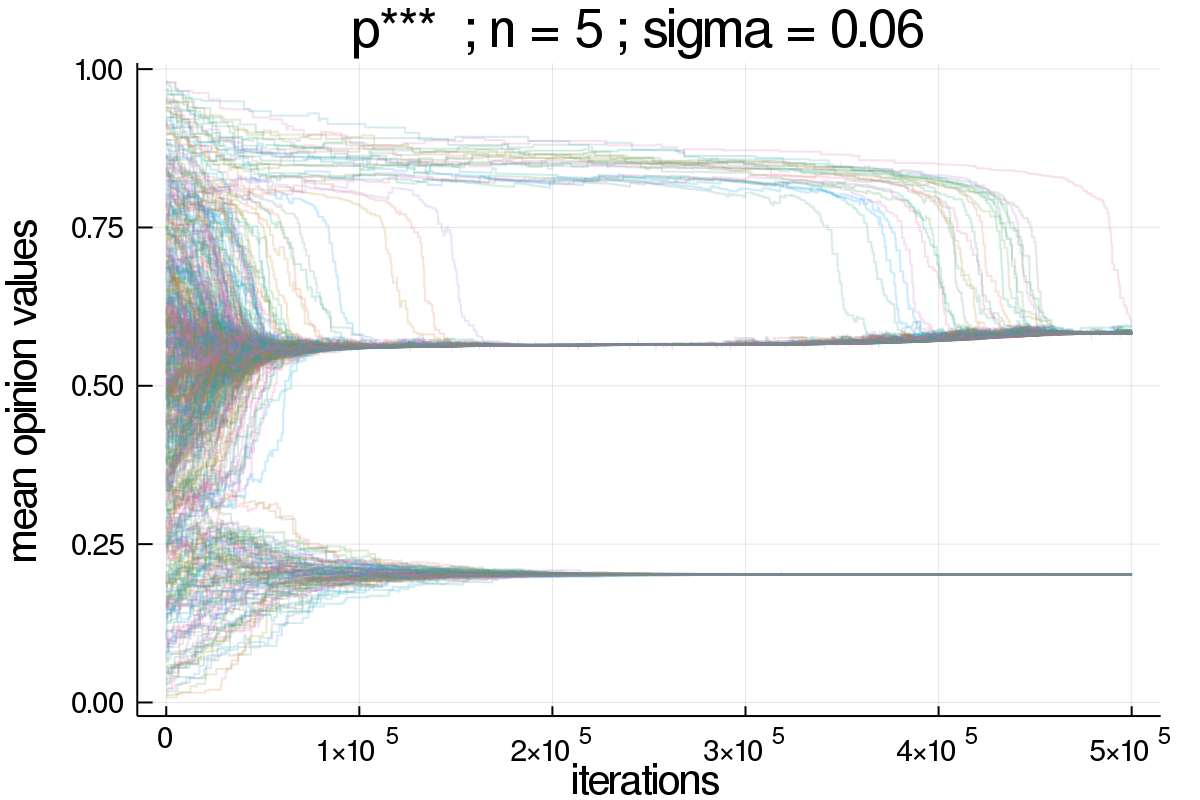
\includegraphics[width=\textwidth]{img/series/tseries6/Poodlcalculatep***n5-rho10e-5-sigma006-00intransrandom.png}
        % \caption{\(n\_issues = 1, \sigma = 0.02\) }
      \end{subfigure}
      \begin{subfigure}[b]{0.49\textwidth}
        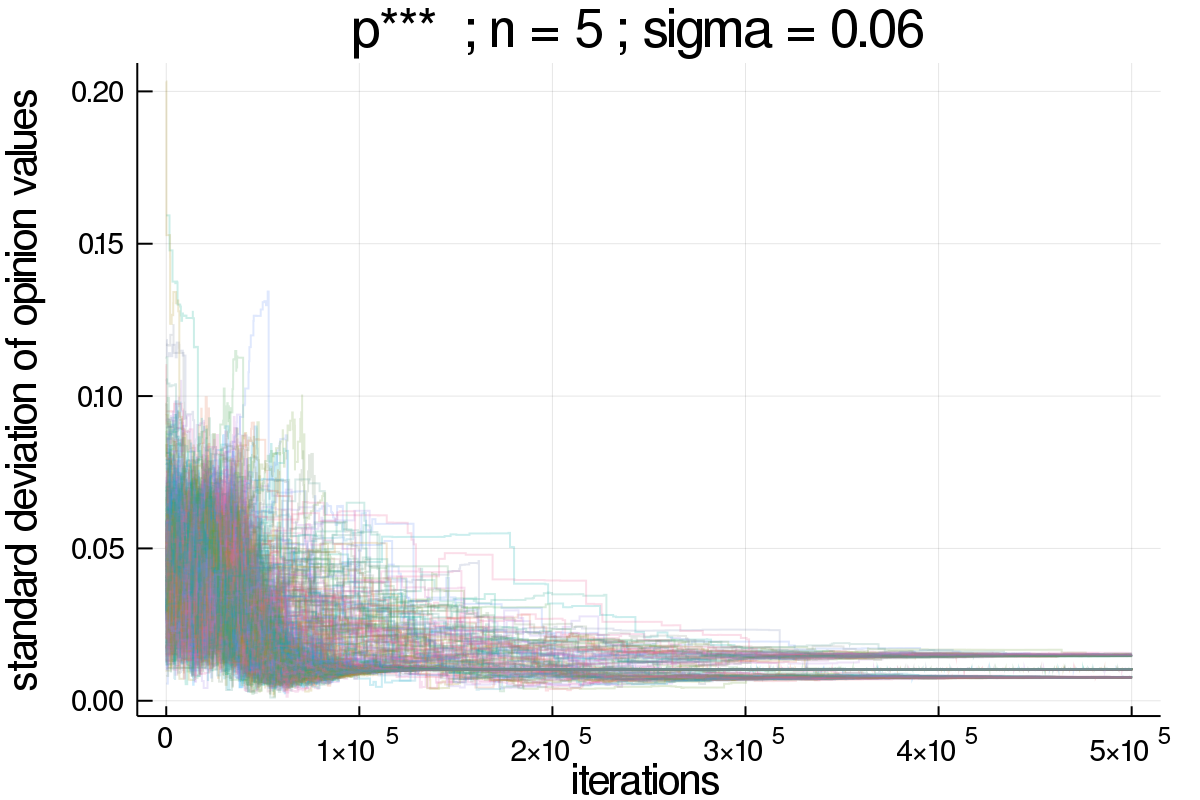
\includegraphics[width=\textwidth]{img/series/tseries6/Poodlcalculatep***n5-rho10e-5-sigma006-00intransrandom-std.png}
        % \caption{\(n\_issues = 1, \sigma = 0.02\) }
      \end{subfigure}
            \begin{subfigure}[b]{0.49\textwidth}
        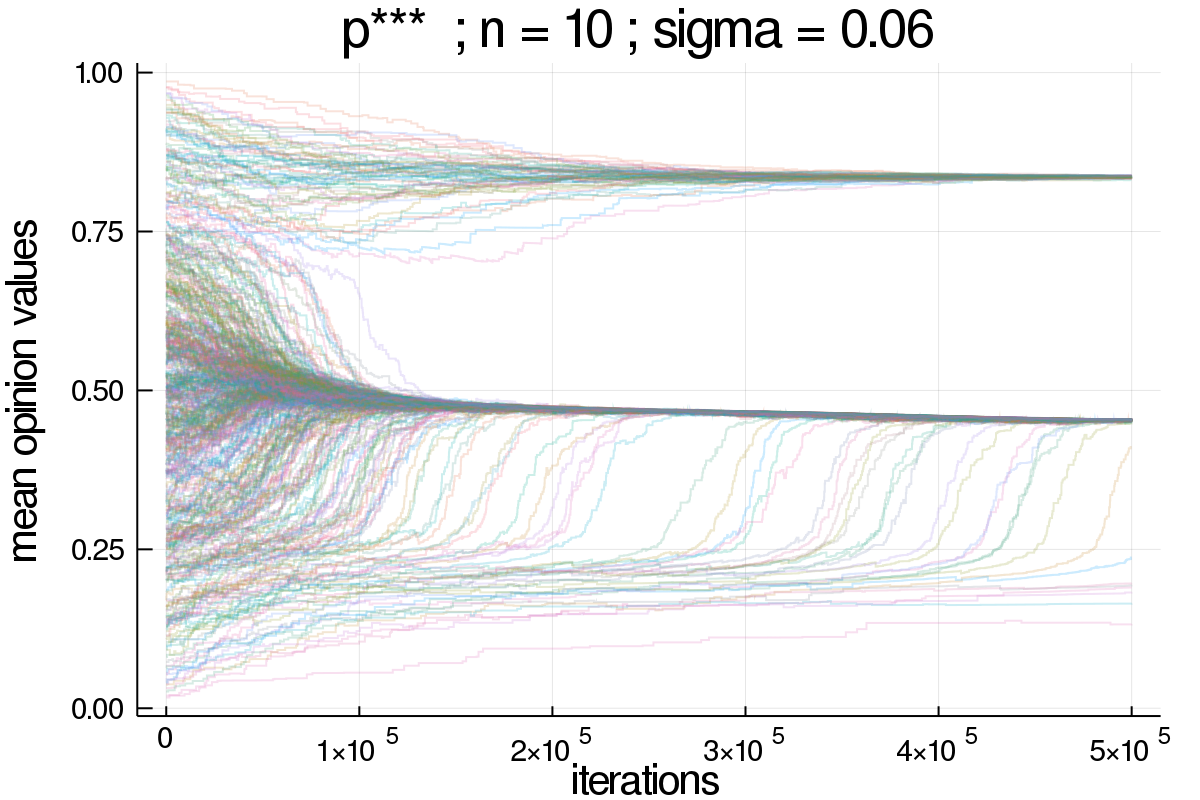
\includegraphics[width=\textwidth]{img/series/tseries6/Poodlcalculatep***n10-rho10e-5-sigma006-00intransrandom.png}
        % \caption{\(n\_issues = 1, \sigma = 0.02\) }
      \end{subfigure}
      \begin{subfigure}[b]{0.49\textwidth}
        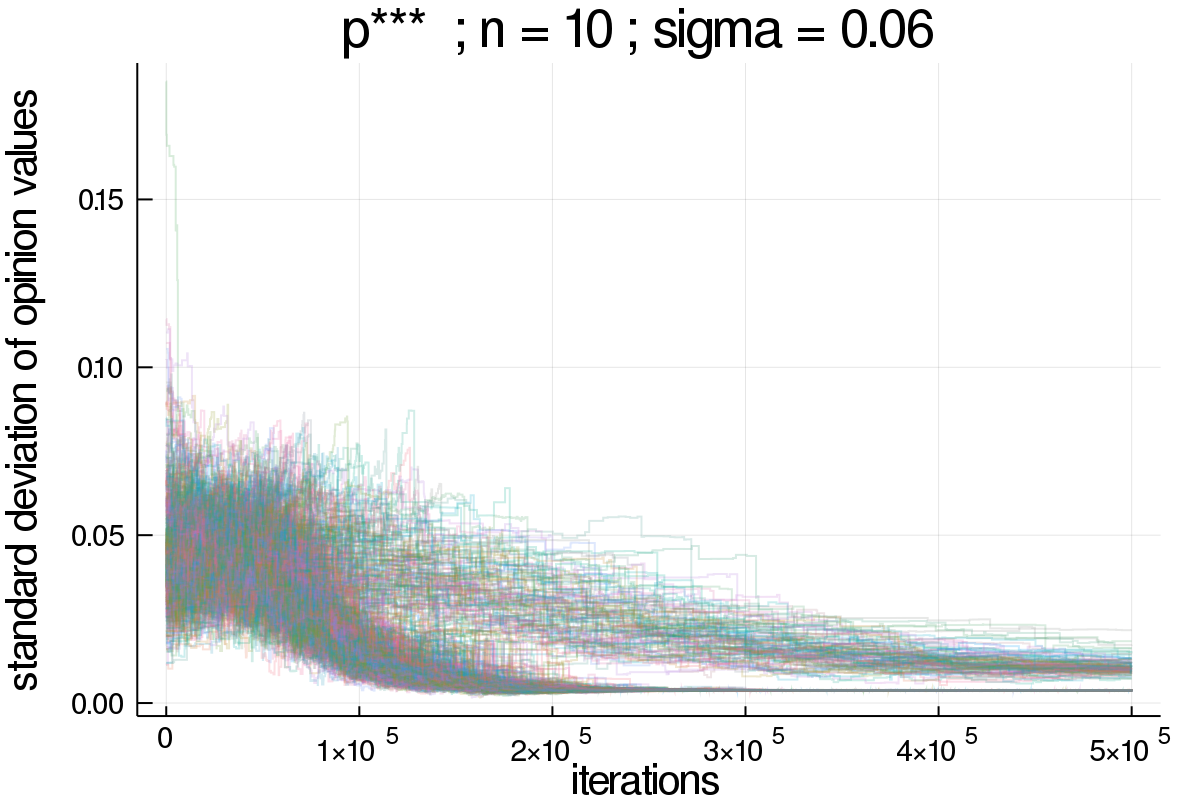
\includegraphics[width=\textwidth]{img/series/tseries6/Poodlcalculatep***n10-rho10e-5-sigma006-00intransrandom-std.png}
        % \caption{\(n\_issues = 1, \sigma = 0.02\) }
      \end{subfigure}
      \caption{Time series for the parameterization: \(\rho = 1e-5, N = 500,
        p\_intran = 0.0 \).}
  \label{fig:tseries6}
    \end{figure}


    \todo[inline, color=yellow!30]{Should I talk about intransigents with
      \(\sigma = 0.01\) ???}
  \section{Conclusions}






\section{Acknowledgement}
The author would like to thank Funda\c{c}\~ao de Amparo \`a Pesquisa do Estado de S\~ao Paulo (FAPESP), for the support to this work, under grant %2008/00383-9.

\bibliographystyle{unsrt}
\bibliography{biblio}

\end{document}

%%% Local Variables:
%%% mode: latex
%%% TeX-master: t
%%% End:
